\documentclass{article} % For LaTeX2e
\usepackage{iclr2025_conference,times}

% Optional math commands from https://github.com/goodfeli/dlbook_notation.
\input{math_commands.tex}




\usepackage[utf8]{inputenc} % allow utf-8 input
\usepackage[T1]{fontenc}    % use 8-bit T1 fonts
\usepackage{hyperref}       % hyperlinks
\usepackage{url}            % simple URL typesetting
\usepackage{booktabs}       % professional-quality tables
\usepackage{amsfonts}       % blackboard math symbols
\usepackage{nicefrac}       % compact symbols for 1/2, etc.
\usepackage{microtype}      % microtypography
\usepackage{xcolor}         % colors
\usepackage{bm}
\usepackage{soul}

\iffalse
% Attempt to make hyperref and algorithmic work together better:
\newcommand{\theHalgorithm}{\arabic{algorithm}}

% Use the following line for the initial blind version submitted for review:

% If accepted, instead use the following line for the camera-ready submission:
% \usepackage[accepted]{icml2023}

% For theorems and such
\usepackage{amsmath}
\usepackage{amssymb}
\usepackage{mathtools}
\usepackage{amsthm}

% if you use cleveref..
\usepackage[capitalize,noabbrev]{cleveref}

%%%%%%%%%%%%%%%%%%%%%%%%%%%%%%%%
% THEOREMS
%%%%%%%%%%%%%%%%%%%%%%%%%%%%%%%%
\theoremstyle{plain}
\newtheorem{theorem}{Theorem}[section]
\newtheorem{proposition}[theorem]{Proposition}
\newtheorem{lemma}[theorem]{Lemma}
\newtheorem{corollary}[theorem]{Corollary}
\theoremstyle{definition}
\newtheorem{definition}[theorem]{Definition}
\newtheorem{assumption}[theorem]{Assumption}
\theoremstyle{remark}
\newtheorem{remark}[theorem]{Remark}


\newcommand{\yongcheng}[1]{\textcolor{orange}{[yongcheng: #1]}}
% Todonotes is useful during development; simply uncomment the next line
%    and comment out the line below the next line to turn off comments
%\usepackage[disable,textsize=tiny]{todonotes}
\usepackage[textsize=tiny]{todonotes}


% The \icmltitle you define below is probably too long as a header.
% Therefore, a short form for the running title is supplied here:
% \icmltitlerunning{Submission and Formatting Instructions for ICML 2023}


% It is OKAY to include author information, even for blind
% submissions: the style file will automatically remove it for you
% unless you've provided the [accepted] option to the icml2023
% package.

% List of affiliations: The first argument should be a (short)
% identifier you will use later to specify author affiliations
% Academic affiliations should list Department, University, City, Region, Country
% Industry affiliations should list Company, City, Region, Country

% You can specify symbols, otherwise they are numbered in order.
% Ideally, you should not use this facility. Affiliations will be numbered
% in order of appearance and this is the preferred way.
\icmlsetsymbol{equal}{*}

\begin{icmlauthorlist}
\icmlauthor{Firstname1 Lastname1}{equal,yyy}
\icmlauthor{Firstname2 Lastname2}{equal,yyy,comp}
\icmlauthor{Firstname3 Lastname3}{comp}
\icmlauthor{Firstname4 Lastname4}{sch}
\icmlauthor{Firstname5 Lastname5}{yyy}
\icmlauthor{Firstname6 Lastname6}{sch,yyy,comp}
\icmlauthor{Firstname7 Lastname7}{comp}
%\icmlauthor{}{sch}
\icmlauthor{Firstname8 Lastname8}{sch}
\icmlauthor{Firstname8 Lastname8}{yyy,comp}
%\icmlauthor{}{sch}
%\icmlauthor{}{sch}
\end{icmlauthorlist}

\icmlaffiliation{yyy}{Department of XXX, University of YYY, Location, Country}
\icmlaffiliation{comp}{Company Name, Location, Country}
\icmlaffiliation{sch}{School of ZZZ, Institute of WWW, Location, Country}

\icmlcorrespondingauthor{Firstname1 Lastname1}{first1.last1@xxx.edu}
\icmlcorrespondingauthor{Firstname2 Lastname2}{first2.last2@www.uk}

% You may provide any keywords that you
% find helpful for describing your paper; these are used to populate
% the "keywords" metadata in the PDF but will not be shown in the document
\icmlkeywords{Machine Learning, ICML}

\vskip 0.3in
]

% this must go after the closing bracket ] following \twocolumn[ ...

% This command actually creates the footnote in the first column
% listing the affiliations and the copyright notice.
% The command takes one argument, which is text to display at the start of the footnote.
% The \icmlEqualContribution command is standard text for equal contribution.
% Remove it (just {}) if you do not need this facility.

%\printAffiliationsAndNotice{}  % leave blank if no need to mention equal contribution
\printAffiliationsAndNotice{\icmlEqualContribution} % otherwise use the standard text.
\fi

% ---- start add by ydu----
\usepackage{graphicx}

\usepackage{subfigure}
% Including math environment
\usepackage{mathrsfs}
\usepackage{amsthm}
\usepackage{amsmath,bm,bbm}
\usepackage{amssymb}
\usepackage{amsmath,amssymb,amsthm}
\usepackage{thmtools}
\usepackage{thm-restate}
\usepackage{tcolorbox}
% \usepackage{comment}
\usepackage{multirow}
\usepackage{tabularx}
\usepackage{multicol}
\usepackage[commandnameprefix=always]{changes}
% \usepackage{xcolor}
% \usepackage[usenames]{color}

% \usepackage[usenames,dvipsnames]{xcolor}

% \usepackage[normalem]{ulem}
%\usepackage[misc]{ifsym}
% \usepackage{natbib}
% \usepackage{colre

% \usepackage{wrapfig}
% \usepackage{graphicx}
\usepackage{amsfonts}
% \usepackage{commath}
\usepackage{url}
\usepackage{mathtools}
% \usepackage{algorithm}
% \usepackage{algorithmic}
% \usepackage[title]{Appendix}
\usepackage{float}
\usepackage{threeparttable}

\newtheorem{mythm}{Theorem}
\newtheorem{mylm}{Lemma}
\newtheorem{mycond}{Condition}
% \newtheorem{mycond}{Condition}[A]
\newtheorem*{myremark}{Remark}
\newtheorem{myprops}{Proposition}
\newtheorem{props}{Proposition}

\newtheorem{mydef}{Definition}
\newtheorem{myasum}{Assumption}
\newtheorem{mycor}{Corollary}
\usepackage{wrapfig}


% Define algorithm env
% using either
\usepackage{algorithm}
\usepackage{algorithmic}
\renewcommand{\algorithmicrequire}{\textbf{Input:}}
\renewcommand{\algorithmicensure}{\textbf{Output:}}
% \usepackage[ruled,linesnumbered]{algorithm2e}

% \DeclareMathOperator*{\argmax}{\arg\,\max}
% \DeclareMathOperator*{\argmin}{\arg\,\min}

\newcommand{\policypi}{\mathbf{\pi} }
\newcommand{\expection}{\mathbb{E} }
\newcommand{\opt}{\mathcal{O}}
\newcommand{\fig}{{Figure }}
\newcommand{\tables}{{Table }}
\newcommand{\eq}{{Eq. }}
\newcommand{\alg}{{Algorithm }}
%\newcommand{\section}{{Sec. }}

\newcommand\blfootnote[1]{%
\begingroup
\renewcommand\thefootnote{}\footnote{#1}%
\addtocounter{footnote}{-1}%
\endgroup
}
% command for comments
\newcommand{\jun}[1]{{\bf \color{red} [Jun: ``#1'']}}
\newcommand{\yanxue}[1]{{ \color{orange}[yanxue: #1]}}
\newcommand{\yan}[1]{{ \color{blue}[yan: #1]}}
\newcommand{\yongcheng}[1]{\textcolor{orange}{[yongcheng: #1]}}
\newcommand{\mengyue}[1]{\textcolor{purple}{[mengyue: #1]}}

% Color{ red, green, blue, cyan, orange, magenta,}

\def\rc{\color{magenta}}
% \usepackage[normalem]{ulem}
\newcommand{\bs}{\boldsymbol}
%\newcommand{\bs}{\mathbf}

\usepackage{changes}
% \usepackage{lipsum}
\usepackage{balance}
\usepackage{tikz-cd}
%----end -- added by ydu--
\iclrfinalcopy
%\title{Probabilistic Decision-Making with Gradient-free Large Language Model Priors}
% \title{Probabilistic inference for Markov Thought Processes with Gradient-free Large Language Model Priors}
\title{Efficient Reinforcement Learning \\with Large Language Model Priors}

% The \author macro works with any number of authors. There are two commands
% used to separate the names and addresses of multiple authors: \And and \AND.
%
% Using \And between authors leaves it to LaTeX to determine where to break the
% lines. Using \AND forces a line break at that point. So, if LaTeX puts 3 of 4
% authors names on the first line, and the last on the second line, try using
% \AND instead of \And before the third author name.


% \author{%
%   David S.~Hippocampus\thanks{Use footnote for providing further information
%     about author (webpage, alternative address)---\emph{not} for acknowledging
%     funding agencies.} \\
%   Department of Computer Science\\
%   Cranberry-Lemon University\\
%   Pittsburgh, PA 15213 \\
  % \texttt{\xue.yan@cs.cranberry-lemon.edu} \\
%   examples of more authors
%   \And
%   Coauthor \\
%   Affiliation \\
%   Address \\
%   \texttt{email} \\
%   \AND
%   Coauthor \\
%   Affiliation \\
%   Address \\
%   \texttt{email} \\
%   \And
%   Coauthor \\
%   Affiliation \\
%   Address \\
%   \texttt{email} \\
%   \And
%   Coauthor \\
%   Affiliation \\
%   Address \\
%   \texttt{email} \\
% }

\author{{\bf Xue Yan$^{~1~2}$ , Yan Song$^{~3}$, Xidong Feng$^{~3}$, 
Mengyue Yang$^{~4}$}\\{\bf Haifeng Zhang$^{\dag~1~2}$, Haitham Bou Ammar$^{~3~5}$, 
Jun Wang$^{\dag~3}$}
\\
\vspace{0.05 cm}\\
{$^1$Institute of Automation, Chinese Academy of Science, Beijing, China}\\
{$^2$School of Artificial Intelligence, University of Chinese Academy of Sciences, China}\\
{$^3$ University College London, UK}
{$^4$ University of Bristol}\\
{$^5$ Huawei Technologies, London, UK}}
% \author{{\bf {Xue Yan$^{~1~2}$,
% Yan Song$^{~1}$, Xinyu Cui$^{~1~2}$, 
% Filippos Christianos$^{~3}$} \\
% \bf {Haifeng Zhang$^{~1}$, 
% David Mguni$^{\dag,3}$, 
% Jun Wang$^{\dag,4}$}}\\
% % \vspace{0.05cm}\\
% {$^1$Institute of Automation, Chinese Academy of Science, Beijing, China}\\
% {$^2$School of Artificial Intelligence, University of Chinese Academy of Sciences, China}\\
% {$^3$ Huawei Technologies, London, UK}
% {$^4$ University College London, UK}}

\begin{document}


\maketitle
\blfootnote{$^\dag$Correspondence to : \textlangle haifeng.zhang@ia.ac.cn \textrangle, \textlangle jun.wang@cs.ucl.ac.uk\textrangle\\}

% \yanxue{Todos: 

% 1. Draw a clear graphic model the inference distribution and posterior distribution.
% \textcolor{red}{MAB done next step: MDP}

% 2. Bellman equation with prior distribution.

% value iteration and policy iteration with prior

% 3. the difference from point-based method for pomdp.


% }

\begin{abstract}
%When humans make complex sequential decisions, they rely on an understanding of the system—a skill developed through experiences in diverse environments, tasks, and learning contexts. However, traditional complex sequential decision-making (SDM) frameworks, such as reinforcement learning (RL) and heuristic search, often require extensive exploration and lack the ability to generalize across varied environments due to a limited understanding of the underlying decision logic. Recently, large language models (LLMs) have achieved significant success as general-purpose tools such as math and decision-making, storing a vast repository of domain-specific knowledge. %Previous studies demonstrate that LLMs can excel in SDM tasks when fine-tuned on task-relevant experience or guided by human-crafted prompts, significantly improving both sample efficiency and generalization. However, these approaches are resource-intensive, limiting their scalability and broad applicability. 

%In this paper, we integrate Large Language Models (LLMs) into Markov Decision Processes (MDPs) from a Bayesian inference perspective, treating LLMs as a prior action distribution. The purpose is to sample from the intractable action posterior that aligns with achieving the desired goals. \yan{\st{We consider two ways to solve the challenge:} This can be done through variational inference or direct posterior sampling with the aim of LLM priors} \st{variational inference and probabilistic sampling, }, implemented within policy-based or value-based RL frameworks. % the This approach requires only the estimation of the likelihood within the LLM prior space, unlike previous methods that rely on fine-tuning LLMs. We estimate this likelihood in both online and offline settings using Q-learning algorithms. 
%Experimental results on ALFWorld and Overcooked demonstrate that incorporating the LLM action prior reduces exploration and optimization complexity compared to traditional policy-based and value-based reinforcement learning, thereby significantly improving sample efficiency.
In sequential decision-making (SDM) tasks, methods like reinforcement learning (RL) and heuristic search have made notable advances in specific cases. However, they often require extensive exploration and face challenges in generalizing across diverse environments due to their limited grasp of the underlying decision dynamics. In contrast, large language models (LLMs) have recently emerged as powerful general-purpose tools, due to their capacity to maintain vast amounts of domain-specific knowledge. To harness this rich prior knowledge for efficiently solving complex SDM tasks, we propose treating LLMs as prior action distributions and integrating them into RL frameworks through Bayesian inference methods, making use of variational inference and direct posterior sampling. The proposed approaches facilitate the seamless incorporation of fixed LLM priors into both policy-based and value-based RL frameworks. Our experiments show that incorporating LLM-based action priors significantly reduces exploration and optimization complexity, substantially improving sample efficiency compared to traditional RL techniques, e.g., using LLM priors decreases the number of required samples by over 90\% in offline learning scenarios.


% Humans rely on accumulated experiences and diverse learning contexts to make complex sequential decisions effectively. In contrast, traditional frameworks for sequential decision-making (SDM), such as reinforcement learning (RL) and heuristic search, often require extensive exploration and struggle to generalize across diverse environments due to a limited understanding of underlying decision dynamics. Large language models (LLMs) have recently demonstrated remarkable success as general-purpose tools, thanks to their ability to store vast repositories of domain-specific knowledge. To leverage these prior knowledge in to solving complex SDM tasks efficiently, we treat LLMs as a prior action distribution and integrate such as LLM Priors into RL framework utilize the a Bayesian inference tools, variational inference or direct posterior sampling. %Our approach enables sampling from the intractable action posterior aligned with achieving desired goals, either through variational inference or direct posterior sampling, 
% This work investigate the incorporation of LLM priors within policy-based or value-based RL frameworks. %To leverage these prior know ledge in solving complex SDM tasks, we propose integrating LLMs into Markov Decision Processes (MDPs) from a Bayesian inference perspective, treating LLMs as a prior action distribution. Our approach enables sampling from the intractable action posterior aligned with achieving desired goals, either through variational inference or direct posterior sampling, leveraging LLM priors within policy-based or value-based RL frameworks. 
% Experimental results on ALFWorld and Overcooked show that incorporating LLM-based action priors reduces exploration and optimization complexity, significantly enhancing sample efficiency compared to traditional RL methods. For example, the engagement of LLM Pirors reduce the examples requirement by at least \textbf{10x} under the offline setting of Overcooked. 
%In this paper, we from a Bayesian inference perspective to integrate the LLMs for SDMs, by treating LLMs as a prior action distribution and analyze the use of LLM priors in Markov Decision Processes (MDPs) from a Bayesian inference perspective, aiming to sample from the intractable action posterior aligned with goal achievement. This approach requires only the estimation of the likelihood within the LLM prior space, unlike previous methods that rely on fine-tuning LLMs. We estimate this likelihood in both online and offline settings using Q-learning algorithms. Experimental results on ALFWorld and Overcooked demonstrate that incorporating the LLM action prior reduces exploration and optimization complexity compared to traditional value-based reinforcement learning, thereby significantly improving sample efficiency.


%Large Language Models (LLMs) have succeeded in complex sequential decision-making (SDM) problems, partly due to their in-context learning and reasoning abilities. Furthermore, high-quality Chain of Thought (CoT) reasoning has proven to enhance the accuracy of actions generated by LLM agents. Previous successes have heavily relied on human-designed prompt engineering, fine-tuned LLM action policies, or extensive search algorithms such as Monte Carlo Tree Search (MCTS). However, these approaches are expensive in terms of human labor and computational resources, which limits their generalization ability. To mitigate these computational expenses, this paper addresses the challenge of effectively utilizing LLMs with CoT for complex SDM tasks. We introduce the concept of Markov Thought Processes (MTPs), which extend standard Markovian decision processes by incorporating a natural language thought space that serves as evidence for inducing precise actions across various environments. We propose a probabilistic inference method to infer latent thoughts and actions according to the structure of the MTPs. This method integrates the online collection of experiences with the prior knowledge possessed by LLMs, thereby enhancing the precision of decisions beyond traditional direct reasoning and action pipelines like ReAct. Moreover, our approach eliminates the need for fine-tuning LLMs or extensive human labor to initiate task-specific CoT reasoning. %. 
%To avoid the heavy computation expenses, in this paper, we explore the pipeline of LLMs with latent thought to address complex SDM challenges and introduce the concept of Markov Thought Processes (MTPs), an extension of standard Markovian decision processes, that incorporate a natural language thought space as the evidence for inducing precises actions in environments. A probabilistic inference method is proposed to infer latent thoughts and actions. This inference procedure combines the online experience collection and LLMs prior knowledge, therefore improve the precious of decisions than LLM directly reasoning and then action pipelines like ReAct. our method reduce uncertainty of LLM agents directly making decision like CoT based ReAct, while do not necciesty fine-tuning LLMs or extensive human-labor for triggering task specific CoT reasoning.%Our approach achieves approximately sampling from the posterior distributions over actions and latent thoughts by integrating the LLM prior with an optimality likelihood estimation derived from environmental feedback. 
%We take the lens of probabilistic inference to tackle complex SDM without the requirement of fine-tuning LLMs, and to explain numerous previous studies on decision-making with LLMs.
%Experimental results demonstrate that our approach, which samples actions from an intricate posterior approximately, can efficiently and effectively solve SDM tasks.







%as well as, These abilities can be further improved via deliberative reasoning strategies, e.g., tree-of-thought prompting.  \textbf{Here, reading the rest first.}


%In addition, deliberative reasoning strategies, such as Chain-of-Thought (CoT) and Tree-of-Thought (ToT), have been demonstrated to further improve the ability of complex reasoning by providing more granular evidence. 

\end{abstract}

%\mengyue{what is the high-quality actions mean in the abstract.  logic begins with fine-tuning LLM very hard and prompts by humans very hard to get, then use that to motivate the generalization ability might have issues. Firstly, the reason why the computationally expensive and latent thought leads to generalization ability is not clear. Then, it's not clear why the LLM latent thought can solve the generalization problem. Why MCTS and CoT is  not enough to solve SDM problem, you still use the LLM based method it also have the computationally expensive problem. The idea is good but the writing still needs to be improved. A better logic might be:  1)background: LLM SDM is important, 2)Problem: MCTS and CoT have huge expenses and low generalization ability. 3) Solution of problem: Use MTPs to reduce the computational expenses by incorporating the Markov process during training, the uncertainty of LLM is only considered as the thought part. and the thought just becomes evidence of the decision, not using the LLM directly to make the decision like CoT. By using this method, we can: 1)reduce uncertainty by using LLM directly to make decisions 2) avoid the high expenses of fine-tuning the LLM 3) Use the knowledge of LLM to enhance the complex decision-making qualities.}


\section{Introduction}
%Various real-world tasks, such as robotics \citep{polydoros2017survey, brunke2022safe, rana2023residual}, autonomous driving \citep{naranjo2005power, song2022quantum}, human-AI dialogue \citep{mctear2022conversational, li2019dialogue}, and human-AI games \citep{yan2024efficient, granter2017alphago}, often involve complex sequential decision-making (SDM) problems. Traditional methods for addressing decision-making problems, such as heuristic search \citep{swiechowski2023monte} and Reinforcement Learning (RL) \citep{mnih2013playing}, have achieved significant success. For instance, AlphaGo \citep{44806} and AlphaStar \citep{vinyals2019grandmaster}, both based on deep reinforcement learning (DRL), have achieved human-level mastery in the games of Go and StarCraft II, respectively. Despite these achievements, traditional methods still face the challenge of requiring extensive interaction with the environment to learn the rules of the world and problem-solving strategies. The need for a large number of samples in each task also limits their generalizability and applicability.


Many real-world tasks, including robotics \citep{polydoros2017survey, brunke2022safe, rana2023residual}, autonomous driving \citep{naranjo2005power, song2022quantum}, human-AI dialogue \citep{mctear2022conversational, li2019dialogue}, and human-AI gaming \citep{yan2024efficient, granter2017alphago}, involve complex sequential decision-making (SDM) challenges. Traditional approaches to SDM, such as optimal control \citep{garcia1989model}, heuristic search \citep{swiechowski2023monte} and reinforcement learning (RL) \citep{mnih2013playing}, have seen substantial success. Notably, AlphaGo \citep{44806} and AlphaStar \citep{vinyals2019grandmaster}, both based on deep reinforcement learning (DRL), have achieved human-level proficiency in the games of Go and StarCraft II, respectively. However, these methods still suffer from high computational complexity, along with poor generalizability and limited applicability across diverse domains \citep{dulac2015deep,cobbe2019quantifying}. %when training from scratch to grasp underlying rules%However, these methods still suffer from high computational complexity or poor generalizability and applicability across diverse domains \citep{dulac2015deep,cobbe2019quantifying}.


% However, these methods still face critical challenges, particularly their reliance on extensive environmental interaction to grasp underlying rules and strategies. Moreover, the high sample complexity in each task often restricts their generalizability and applicability across diverse domains.






%Recently, Large Language Models (LLMs) have emerged as effective tools for tackling diverse general-purpose tasks, such as in dialogue systems \citep{brooks2023large}, decision-making \citep{zhao2024expel}, and mathematical reasoning \citep{imani2023mathprompter}. Their impressive performance across various domains is largely attributed to the vast amounts of human knowledge they compress during the pre-training phase on extensive corpora \citep{tucker2023increasing}. Several studies explored utilizing LLMs to solve long-term sequential decision-making (SDM) tasks by human-crafted prompt-engineering or fine-tuning on extensive interactive experience with each environment. The prompt-engineering approaches, known as LLM-Agent, e.g., Proagent \citep{zhang2023proagent} on overcooked, and Voyager \citep{wang2023voyager} in Minecraft, rely on high-quality human-designed prompts for step-by-step successful action generation. %The work in \citep{christianos2023panguagent} then introduced an intrinsic functions framework that unified prompting techniques and demonstrated successful results in embodied environments like Alfworld \citep{Alf}. 
%These methods are labor-intensive, requiring task-specific prompt design from expert humans, limiting their generalization ability. Of course, the other works \citep{carta2023grounding,jang2021gpt,wen2024entropy,yan2023ask,zhou2024reflect} attempted finetuning-based approaches to boost the LLM's performance in such domains; see Section \ref{Sec:RelatedWork} for a detailed exposure of related work. For instance, each of GFLAN \citep{carta2023grounding}, GPT-critic \citep{jang2021gpt}, and the Pangu-Agent \citep{christianos2023panguagent} leverage RL fine-tuning of LLM action policies to solve long-horizon decision-making problems. While fine-tuning methodologies boost performance by tailoring the pre-trained priors encoded in LLMs through task-specific experiences gathered in the environment. 

{
    Recently, Large Language Models (LLMs) have emerged as effective tools for tackling diverse general-purpose tasks, such as in dialogue systems \citep{brooks2023large}, decision-making \citep{zhao2024expel}, and mathematical reasoning \citep{imani2023mathprompter}. Their impressive performance across various domains is largely attributed to the vast amounts of human knowledge compressed during the pre-training phase on extensive corpora \citep{tucker2023increasing}. %Traditional neural network-based decision-making agents typically require training from scratch to grasp underlying rules and are weak in reusing experience across tasks or leveraging human prior knowledge. 
    Inspired by how humans make decisions using existing knowledge while learning from new tasks, LLM-based agents are emerging as a promising approach for solving SDM tasks. For instance, researchers leverage human-crafted prompts to guide LLMs in making decisions directly \citep{zhang2023proagent, wang2023voyager, ma2023large}. While this approach relies heavily on the quality of the prompts and the LLMs' inherent capabilities, another line of research aims to fine-tune LLMs with RL algorithms (RLFT) \citep{carta2023grounding, christianos2023panguagent,tantrue,zhou2024reflect} to enhance their decision-making precision. A more detailed exploration of related work can be found in Section \ref{Sec:RelatedWork}. However, these approaches are resource-intensive, as they require meticulously crafted human prompts and an expensive fine-tuning process for LLMs for each specific task.

 %However, these works do not fully leverage the rich prior knowledge encapsulated in LLMs while being subjected to the notorious drawbacks of RL at the same time. 
% reinforcement learning methods are notorious for their high computation complexity training from scratch and sensitivity to high dimensional action space \citep{dulac2015deep}. }

%In decision-making contexts, researchers have either designed human-crafted prompts to guide model actions directly \citep{zhang2023proagent} or employed complex reward models to shape behavior in environments \citep{snell2024scaling}. 

}



%Inspired by the above successes, we aim to combine the benefits of rich domain knowledge, which is encapsulated in LLMs, with the strengths of RL algorithms in learning problem-solving rules. While it is challenging for LLMs to solve sequential decision-making (SDM) tasks in a zero-shot manner due to the lack of task-specific domain knowledge and interactive experience, they can still generate suboptimal actions given a state \citep{zhang2024can}. To effectively leverage the potential of large language models (LLMs) in sequential decision-making (SDM) tasks, we treat the LLMs as a prior action distribution and analyze their impact on solving Markov Decision Processes (MDPs) from a Bayesian inference perspective \citep{hu2023amortizing}. The overall objective is to compute the posterior action distribution consistent with the goal achievement condition. However, such a desirable posterior action distribution is often intractable. There are two commonly used probabilistic approaches to approximate the posterior distribution: variational inference and probabilistic sampling. Following the derivation from \citep{levine2018reinforcement}, the probabilistic inference approach, known as Control as Inference, is shown to be related to the classical RL framework, therefore RL is an effective and robust tool for implementing posterior inference. We will describe the realization of variational inference and probabilistic sampling by combining RL and suboptimal LLM priors below.


Inspired by these, this work stands in the position of combining the advantages of leveraging rich domain knowledge with the strengths of reinforcement learning (RL), but in a different perspective to use fixed LLMs to enhance traditional RL.
%Another line of research seeks to combine the advantages of leveraging rich domain knowledge with the strengths of reinforcement learning (RL) \citep{carta2023grounding}, which is where our approach is positioned. 
The key insight is that while it may be challenging for an LLM to generate optimal plans at every state with limited experience, it can still offer suboptimal action proposals or significantly reduce the size of the action space to a manageable scope, thereby alleviating computational burdens. Building on this idea, we treat the LLM as an action prior distribution and incorporate it into Markov Decision Processes (MDPs) solving from a Bayesian inference perspective \citep{hu2023amortizing}. The primary objective is to approximate the posterior action distribution that aligns with task goals through probabilistic inference approaches such as variational inference or direct posterior sampling. Building on these approaches, we derive the incorporation of LLMs into both policy-based and value-based RL frameworks in a simple yet logically sound manner. We conduct experiments on major benchmarks like ALFWorld and Overcooked, demonstrating that the sample efficiency of traditional RL algorithms, such as value-based DQN and policy-based PPO, can largely benefit from integrating LLM action priors.%Building on this idea, we treat the LLM as an action prior distribution and incorporate it into Markov Decision Processes (MDPs) from a Bayesian inference perspective \citep{hu2023amortizing}. The primary objective is to approximate the posterior action distribution that aligns with task goals through probabilistic inference techniques such as variational inference or sampling methods. We conduct experiments on major benchmarks ALFWorld and Overcooked and show that the sample efficiency of traditional RL algorithms, such as value-based DQN and policy-based PPO, can largely benefit from integrating LLM action priors.

% In this paper, we explore these techniques within the RL framework, leveraging a fixed LLM to generate suboptimal action proposals, which helps improve sample efficiency. By integrating LLM action priors, we propose simple yet efficient policy-based and value-based RL algorithms. We conduct experiments on ALFWorld and Overcooked \yan{\st{to evaluate the advantages of integrating language priors within RL frameworks.} and show that the sample efficiency of traditional RL algorithms, such as value-based DQN and policy-based PPO, can largely benefit from integrating LLM action priors.}



% \yan{Delete this paragraph? or move to related work}Note that, compared to previous prompt-engineering-based LLM agents and RLFT approaches, we propose a simple yet efficient value-based RL algorithm for LLMs to solve complex SDMs in a bootstrap manner while eliminating the expensive human-crafted prompt design and fine-tuning of LLMs. The LLM prior acts in reduce the original action space, therefore significantly improve the simple efficiency in online and offline settings. Additionally, several studies \citep{feng2023alphazero, yao2024tree, hao2023reasoning} on improving LLMs' reasoning ability also fit the posterior sampling framework by using value estimation of reasoning traces to guide the selection of the next step reasoning output from LLMs.  However, our work utilizes more efficient TD-learning for value estimation, in contrast to the heuristic search-based planners and LLMs as evaluator used in previous work.


In summary, our main contributions are three-fold:
\begin{enumerate}
    % \item We incorporate the Large Language Model into the reinforcement learning framework and formulate it from a Bayesian view. \yan{more on the theoretical side?}
    % \item We propose simple yet efficient value-based RL algorithms using fixed LLM to generate action proposals.  \yan{not proposing, emphasis plug-and-play}
    % \item We explore the advantages of integrating the LLM prior into value-based RL in both online and offline settings. \yan{generalization of value function?}
    \item {We present a unified framework for integrating Large Language Models (LLMs) as probabilistic priors into Markov decision-making frameworks. \textbf{(Section \ref{sec: method})}
} %In this context, the primary objective is to model the posterior distribution under the assumption of optimality and plan through inference. 
    \item {We practically implement the framework by leveraging LLMs as the refined action sampler for value-based online RL \textbf{(Section \ref{sec: online_value_rl})}, offline RL \textbf{(Section \ref{sec: offline_value_rl})} or behavior regularizer for policy-based RL \textbf{(Section \ref{sec: online_policy_rl})}.}
    %\yan{We present a unified approach for integrating Large Language Models (LLMs) as probabilistic priors within Markov decision-making frameworks. In this context, the primary objective is to model the posterior distribution under the assumption of optimality and plan through inference. LLMs can function either as behavior regularizers or refined action samplers, leveraging their rich prior knowledge to guide the learning process more effectively.}
    %\item \yan{We present a unified approach for integrating Large Language Models (LLMs) as probabilistic priors within Markov decision-making frameworks. In this context, the primary objective is to model the posterior distribution under the assumption of optimality and plan through inference. LLMs can function either as behavior regularizers or refined action samplers, leveraging their rich prior knowledge to guide the learning process more effectively.}
    % \yan{\st{We frame sequential decision-making tasks as Bayesian inference problems and incorporate Large Language Models as a prior distribution in the context.}}
    % \item We discuss practical ways to use LLM to propose refined decision subspace and perform efficient reinforcement learning algorithms.
    % %\item 
    % \item We carry out experiments on both online and offline settings, investigating the advantages of integrating a LLM as a prior distribution.
    \item {Extensive experiments on ALFWorld and Overcooked demonstrate that our new framework can significantly boost sample efficiency compared with both pure RL and pure LLM baselines, and also bring in more robust and generalizable value function. \textbf{(Section \ref{sec: exp})}}
    
    
    % \yan{\st{We discuss practical ways to use LLM to improve tradition RL frameworks. Experiments in both online and offline settings demonstrate a significant improvement in sample efficiency compared to traditional RL. 
    % Notably, the offline learning experiments on Overcooked show that incorporating LLM action priors can improve sample efficiency by \textbf{10x}.} \yan{We explore practical approaches for using LLMs } 
    %We carry out experiments on both online and offline settings, investigating the advantages of integrating LLM action priors. 
    % \item \yan{Things we have done + conclusion} Integrating LLM priors into value-based RL allows us to generalize to larger or smaller-scale LLMs, achieving superior performance or reducing distribution complexity during inference.

    
    %We carry out experiments on both online and offline settings, investigating the advantages of integrating LLM action priors. 
    %We conduct experiments in both online and offline settings, exploring the advantages of integrating LLM action priors. 
    %Notably, the offline learning experiments on Overcooked show that incorporating LLM action priors can improve sample efficiency by \textbf{10x}. 
    % Integrating LLM priors into value-based RL allows us to generalize to larger or smaller scale LLMs, achieving superior performance or reducing distribution complexity during inference. %The value-based RL with LLM prior enable us to generalize to larger or smaller scale LLM for superior performance or reduce. distributed difficulty
%Experiment results demonstrate the effectiveness of integration of the LLM prior in improving sample efficiency in both policy-based and value-based RL.
\end{enumerate}

\iffalse


For the variational inference solution, we need to learn a parametric policy (that can generate an action distribution) to approximate the intractable posterior action distribution. This is achieved by maximizing the cumulative reward while minimizing the distance between the optimized policy and the LLM prior policy, measured by the Kullback-Leibler (KL) divergence. Regularizing the policy to be similar to the LLM prior policy encourages the action policy to distill task-relevant prior knowledge from the powerful LLMs, thereby reducing meaningless exploration. Since a parametric action policy is required, it is natural to implement the variational inference with an LLM as the prior using policy-based RL fine-tuning. Note that to fully use the human knowledge of pre-trained language model\citep{zhou2024reflect,tantrue}, the policy-based RL is conducted by fine-tuning a small LM-based action policy as GFlan \citep{carta2023grounding}.




%Similar to standard NLP reasoning tasks, such planning techniques can improve in SDM domains via well-crafted prompts that trigger the LLM policy to produce valid chains of thought \citep{huang2024understanding,stechly2024chain}, leading to effective per-step actions, e.g., high-level subgoals that, if sequenced correctly, solve the overall high-level task. However, the challenge of crafting prompts that trigger effective CoTs for long-term sequential decision-making tasks is formidable due to the vast state space and the multifaceted skills these tasks demand, including exploration, learning from experience, and exploitation capabilities. 


The variational inference approach requires fine-tuning even a small LLM policy, which is computationally expensive. To avoid fine-tuning a language model, we attempt to realize the approximate posterior sampling, by involving the optimality likelihood and the LLMs prior. Specifically, the optimality likelihood is estimated based on environmental interactions and is associated with high cumulative rewards (e.g., episodic Q-values in MCTS \citep{hao2023reasoning}). This likelihood is then used to reweight decisions from the prior, providing an "approximation" to the posterior. Several studies \citep{yao2024tree, feng2023alphazero} that enhance the LLM reasoning ability follow this process as an instance of probabilistic inference, where posterior reasoning steps are sampled from LLM priors after estimating the current trace values, which act as likelihoods.  
%follow previous work and utilize inference-time planners. However, we notice that currently available solvers are highly computationally and time-intensive. For example, MCTS-based decoders require many calls to the LLM, while BFS and DFS strategies blow up in large state and action spaces. Abstracting these related works to understand their limitations, we observe that most inference-time algorithms are, in fact, considering the LLM as a prior due to its powerful reasoning abilities with the hope of effectively exploring complex SDM tasks compared to tabula-case reinforcement learning. The likelihood estimation from environmental interactions (e.g., episodic Q-values in MCTS \citep{hao2023reasoning}) then reweighs decisions from those priors providing an ``approximation'' to the posterior. We formalize this process as an instance of probabilistic inference in which posterior actions are sampled from LLM priors after estimating cumulative environmental rewards which act as likelihoods. Therefore, determining the right action sequence that maximizes rewards can now be targeted from a probabilistic inference perspective in which we must sample from \emph{intractable posterior policies} - the result of the product between optimality likelihood estimates and LLM action and thought priors. We handle this inference problem in two steps. The first approximates the likelihood of success, while the second approximately samples from the posterior action distribution. 

%When approximating the likelihood of success, we note several options that can be derived as special cases when considering different estimation methods. For example, heuristic search-based planners \citep{feng2023alphazero} or LLM as an evaluator \citep{yao2024tree, zhang2024can}, however, these approaches are heavy in interactive samples or mediculous human-labor requirements.  
When approximating the likelihood of success, we note several options that can be derived as special cases when considering different estimation methods. For example, \citep{feng2023alphazero,hao2023reasoning} use heuristic search-based planners or  \citep{yao2024tree, zhang2024can} let LLMs as evaluators. However, these estimation approaches often require a large number of interactive samples or meticulous human labor.
%suppose we use Q-value statistics of a complete episode as our likelihood estimator. In that case, we can recover MCTS-based planners, while if we consider the LLM as an evaluator, we recover a tree-of-thought- like strategy. 
Since Q-values are positively associated with optimality in a given state-action pair, 
we opt to employ temporal difference learning \citep{tesauro1995temporal} as a computationally more efficient estimate of the success likelihood. We recruit DQN and CQL algorithms within the LLM prior action space for Q-value estimation in both online and offline settings. To represent the Q-network, we introduce an adapter on top of the LLM embeddings and fit the adapter's weights by minimizing the temporal difference loss. Our LLM is frozen during this step, and we do not propagate any gradients to avoid additional computational overhead. 
\fi
%Given the updated adapter, we still require an algorithm that samples actions from our intractable posterior. Of course, this can be approached from variational inference, where we approximate intractability by a variational distribution. While being a viable option, variational distributions for MTPs need to be language models themselves that accept natural language states and actions; thus tuning them requires extra gradient steps in large models. We avoid those additional computations by proposing a thought and action sampling strategy that samples thoughts and actions from prior LLMs and scores them according to ... \textcolor{red}{H: To continue we need exp results now to see which option works best}  

%While we can follow a variational inference approach \citep{VIBlie} to tackle the posterior's intractability, 
 
%Interestingly, our formulation unifies other planning strategies that  

 


%\textbf{Here}
%Inspired by the success of LLMs in complex NLP tasks, several studies also explore utilizing them to solve long-term decision-making tasks. For example, prompt engineering-based method Proagent \citep{zhang2023proagent} for Overcooked and Voyager \citep{wang2023voyager} for Minecraft with human deliberately designed prompts for step-by-step action generation. 
%Furthermore, finetuning-based methods such as Gflan \citep{carta2023grounding} and GPT-critic \citep{jang2021gpt} also utilize the reinforcement learning (RL) algorithm and LLMs served as the backbone of the action policy to be fine-tuned, 

%On another front, finetuning-based approaches like GFLAN \citep{carta2023grounding} and GPT-critic \citep{jang2021gpt} leverage reinforcement learning (RL) algorithms with LLMs serving as the action policy. 
% these methods benefit from both the rich world knowledge prior contained in the LLM action policy as well as collect task-oriented the experience collected from interactive with environments, however, but fine-tuning this LLMs action policy requires expensive computational cost.   

%To avoid expensive finetuning on LLM action policies for decision-making tasks, designing a deliberate planning strategy is an important alternative to improving the quality of actions generated from LLMs. 


%Numerous studies have explored the path of utilizing pre-trained and fixed LLMs with elaborate planning techniques to figure out complex decision-making tasks. For instance, the Tree of Thought (ToT) \citep{yao2023tree} and RAP utilises the BFS/DFS search algorithms, and the MCTS \citep{browne2012surveymonte,ellis2019write,huang2024understanding,zeng2023large} to plan the accurate decision(action) sequence based on LLM assessments. %, and the RAP \citep{hao2023reasoning} uses the MCTS \citep{browne2012surveymonte} to guide the step-by-step solution reasoning process. 
% These approaches all take effort to find desirable action sequences in the long-term decision-making process. 
%Despite various attempts to integrate fixed LLMs with planning strategies for decision-making, a systematic and unified explanation is still lacking to epitomize those previous approaches. In this work, we propose a unified probabilistic inference framework for decision-making tasks with LLM prior, we view the desirable action planning based on LLM prior as an intractable posterior inference problem. Concretely, at each state ss, the posterior distribution across (natural language type) action aa conditioned on the optimality condition is required: 
%\begin{equation}
%\label{posterior}
%p(a|s,\mathcal{O}=1)=\frac{p(\mathcal{O}=1|a,s)p(a|s)}{p(\mathcal{O}=1|s)},
%\end{equation} where O\mathcal{O} is the random variable that indicates the optimality of a trajectory. %The optimality, referring to the control as inference for traditional RL \citep{abdolmaleki2018maximum}, means, for example, completing a task or accurately answering a question. 
%The optimality O=1\mathcal{O}=1, referring to the control as inference in traditional RL \citep{abdolmaleki2018maximum}, implies successful completion of a task or precise answering of a question. %Despite these attempts, it is still worth noting that the posterior distribution over the action sequence is intractable. 
%As shown in \eq (???)(???)(???)(???)\eqref{posterior}, the intractable action posterior can be approximated by integrating the gradient-free LLM prior with the optimality likelihood estimation, thus it benefits from both the unnecessary of finetuning LLMs and the task-specific experience reflected in the likelihood. There exist different optimality likelihood estimation methods, for example, LLM assessment in ToT and Q-value statistics during MCTS in RAP. %In this work, we assume that the Q-value is positively correlated the optimality likelihood under the current state and action, and then naturally use TD-learning to learn the Q-value with the state-action embedding from LLMs as the Q-function's input. 
%In this work, we posit that the Q-value is positively associated with the optimality likelihood under a given state-action pair. Consequently, we naturally employ Temporal Difference (TD) learning \citep{tesauro1995temporal} to estimate the Q-value, using the state-action sentence embeddings derived from LLMs as inputs to the Q-function. It is also worth noting that, most of previous studies on LLMs for decision-making can also be interpreted in our framework, which is detailed illustrated in Table ???????????????????????????\ref{tab:summary}.% which estimate the likelihood using LLM assessment and MCTS Q-value estimation.


% To achieve the purpose of finding the optimal per-step action based on gradient-free LLMs prior, on the one hand, we consider using Bayesian inference to approximate the more precise action posterior. On the other hand, we consider using the CoT reasoning to further improve the quality of LLM prior to generate actions. 
% %Besides the trajectory level action discovery based on the task completion condition, we also consider using the CoT reasoning to further improve the quality of the action reasoning. 
% Inspired by the successful evidence of CoT reasoning in enhancing the mathematical and logical reasoning solving ability, we think the intermediate CoT reasoning could also be helpful for per-step action generation. For example, in the Overcooked game, %directly determine the correct sequence of actions is difficult, however, LLMs compressed human knowledge can plan the high level solution for successful deliver a dish. 
% LLMs is struggle to directly determine a correct fine-grained action sequence, but it is simpler for LLMs to first plan a sequence of the high level subgoals, for example, take an onion, then cut it, then put it on a plate, then serve. According to the intermediate subgoal guidance, the LLMs is more likely to succesfully acheive the final goal. The process of the action generation with CoT reasoning can be represented as: p(a|s)=∑υp(a,υ|s)=∑υp(a|s,υ)p(υ|s)p(a|s)=\sum_\upsilon p(a,\upsilon|s)=\sum_\upsilon p(a|s,\upsilon)p(\upsilon|s), where we treat the intermediate thought as a latent variable υ\upsilon. The traditional CoT reasoning approach directly generate the latent thought from the prior p(υ|s)p(\upsilon|s) via prompt engineer. However, the intractable posterior p(υ|s,O=1)p(\upsilon|s,\mathcal{O}=1) is more desirable than the prior. Consistent with the action inference in \eq (???)(???)(???)(???)(???)(???)(???)(???)(???)(???)(???)(???)\eqref{posterior}, we also use the Bayesian inference method to figure out sampling from the intricate posterior distribution.  

%To find the optimal action at each step based on gradient-free LLM priors, we approach this from two directions. Firstly, we utilize Bayesian inference to approximate the more precise action posterior. Secondly, we incorporate CoT reasoning to refine the quality of action generation. Drawing inspiration from CoT reasoning's successful enhancement of mathematical and logical reasoning capabilities, we hypothesize that intermediate CoT reasoning steps could also be beneficial for determining per-step actions. For instance, in the Overcooked game, although LLMs might struggle to directly deduce the correct fine-grained action sequence, they can effectively outline high-level subgoals. For example, LLMs can figure out the subgoals pick up an onion, cut it, place it on a plate, and serve. By following the guidance of these intermediate subgoals, LLMs become more capable of achieving the final objective. This action generation process with CoT reasoning can be mathematically depicted as: $p(a|s) = \sum_\upsilon p(a, \upsilon|s) = \sum_\upsilon p(a|s,\upsilon)p(\upsilon|s).Here,wetreatintermediatethoughtsaslatentvariables. Here, we treat intermediate thoughts as latent variables \upsilon.TraditionalCoTreasoningmethodsgeneratetheselatentthoughtsfromtheLLMprior. Traditional CoT reasoning methods generate these latent thoughts from the LLM prior p(\upsilon|s)usingpromptengineeringtechniques.However,theintractableposterior using prompt engineering techniques. However, the intractable posterior p(\upsilon|s, \mathcal{O} = 1)$, which considers optimality, is more valuable than the prior alone. In line with the action inference outlined in Eq. (1), we also apply Bayesian inference to sample from this complex posterior distribution. 
% For traditional NLP tasks such as mathematical and logical reasoning problems, the emergence of high-quality CoT reasoning usually relies on human carefully designed prompts. However, for more complex decision-making tasks, the human-crafted prompt design is more difficult due to the large state space and the complicated skills its required ranging from exploration and learn and exploit skills.
%In conventional NLP tasks, such as mathematical and logical reasoning, the emergence of high-quality CoT reasoning often stems from meticulously crafted human prompts. Conversely, in more intricate long-term decision-making tasks, crafting effective prompts becomes exceedingly challenging due to the vast state space and the multifaceted skills these tasks demand, including exploration, learning from experience, and exploitation capabilities. When we obtain a CoT prompt set C\mathcal{C}, this action generation process with CoT reasoning can be mathematically depicted as p(a,υ|s,C)=p(a|s,υ)p(υ|s,C)p(a,υ|s,C)=p(a|s,υ)p(υ|s,C)p(a,\upsilon|s,C)=p(a|s,\upsilon)p(\upsilon|s,C)p(a,\upsilon|s,\mathcal{C})=p(a|s,\upsilon)p(\upsilon|s,\mathcal{C}). Here, we treat intermediate thoughts as latent variables υ\upsilon. We denote the decision-making process with the latent thought to assist in action performing as the Markov Thought Decision Making Process (MTDP). Previous studies design a CoT prompts set in a human-crafted manner \citep{wei2022chain,lin2024swiftsage} mathematically written as phuman(C|task descriptions)p_\text{human}(\mathcal{C}|\text{task descriptions}). In this work, we are more interested in the intractable posterior over the prompts set p(C|O=1)p(C|O=1)p(C|O=1) p(\mathcal{C}|\mathcal{O}=1), which indicates the task-specific prompt hints condition on the optimality. In line with the action inference outlined in Eq. (???)(???)(???)\eqref{posterior}, we also apply the Bayesian inference tool to realise that approximately sample from this complex posterior distribution.
%Our motivations are threefold:

% Firstly, we from the probabilistic inference perspective to work out the decision-making tasks, concretely we utilise the LLMs prior to inferece and approximate actions and thoughts posterior in MDPs, without relying on policy gradient methods on LLMs policies. Applying probabilistic inference methods brings benefits such as unnecessary on expensive LLM prior finetuning and usage of well-known Bayesian inference technique for accurate posterior approximation.


% Secondly, we incorporate language thought into the MDP framework, which enhances performance of LLMs on tackling complex decision-making tasks with more task-relavent latent evidence provided.


\iffalse
In summary, our contributions are three-fold:

Firstly, we adapt the probabilistic inference perspective to effectively incorporate the LLM as a valuable action prior to address decision-making tasks. 

Secondly, we propose simple yet efficient RL algorithms to approximate the intractable action posterior from both the variational inference and probabilistic sampling perspectives.

Thirdly, we demonstrate the effectiveness of the LLM prior in improving sample efficiency in both policy-based and value-based RL.
\fi

\iffalse

\section{Preliminary}
\label{pre}
We first introduce the formulation of the Markov Decision Process (MDP) as well as the value-based reinforcement learning (RL) algorithm in both online and offline settings.


% This section introduces the Markov Decision Process (MDP) formulation and representative online and offline value-based Reinforcement Learning (RL) algorithms. Additionally, we present a probabilistic perspective to explain the LLMs as action priors.
% In order to improve the performance of pre-trained LLMs on directly executing on the decision-making tasks, we formulate the MDPs-solving problem with LLMs as a Bayesian Inference problem, as well as incorporating latent thought to guide the action generation. %This work investigates how to add the language before MDP to improve MDP's representation ability.

\paragraph{Markov Decision Process}
A Markov Decision Process (MDP) can be described as a tuple $\langle\mathcal{S},\mathcal{A},P,r,\gamma\rangle$. $\mathcal{S}$ is the state space, and $\mathcal{A}$ is the finite action space. We consider the textual action space and state space here. Each state $s$ and each action $a$ is a sentence $s,a\in \mathcal{V}^\infty$, where $\mathcal{V}$ is the vocabulary set. $P:\mathcal{S}\times\mathcal{A}\rightarrow \Delta(\mathcal{S})$ is the transition kernel, mapping the current state $s_t$ to the next state $s_{t+1}$ following the action $a_t$. $r:\mathcal{S}\times\mathcal{A}\rightarrow \mathbb{R}$ is the reward function. $\gamma$ is the discount factor. %If under the partial observation setting, the partially observable Markov Decision Process (MDP) is described with $\langle\mathcal{S},\mathcal{A},P,r,\gamma,\mathcal{O}\rangle$. 
 %$\mathcal{O}$ is the observation space, $P(o|s)$ note the probability of the observation $o\in\mathcal{O}$ is visiable under the state $s\in \mathcal{S}$. The objective function for the POMDP is written as:  $\pi^*\in \arg\max _\pi \mathbb{E}_\pi[\sum_t \gamma^t r(s_t,a_t)|a_t \sim \pi(\cdot|o_t), o_t\sim P(\cdot|s_t)]$
The objective of RL for solving an MDP is to learn an action policy $\pi(a|s)$, such that maximize the discounted cumulative reward $\pi^*=\arg\max_\pi \mathbb{E}_{p_\mathcal{A}(\theta)}[\sum_t \gamma^t r(s_t,a_t)|a_t \sim \pi(\cdot|s_t)]$.
\fi
\iffalse
Since we aim to use LLMs to solve the MDP, the action policy $\pi(\cdot|s)$ is indeed an action LLM denoted as $p_\mathcal{A}(\cdot|s;\theta)$, and the action is sampled from the LLM in the autoregressive manner $a\sim p_\mathcal{A}(\cdot|s;\theta)$. 
The general RL algorithm usually aims to learn an action policy $p_\mathcal{A}(\cdot|s;\theta^*)$ such that maximize the cumulative discounted reward, formally written as: $\theta^*\in \arg\max _\theta \mathbb{E}_{p_\mathcal{A}(\theta)}[\sum_t \gamma^t r(s_t,a_t)|a_t \sim p_\mathcal{A}(\cdot|s_t;\theta)]$.
\fi

\section{Formulation}
\label{sec: method}
%This work seeks to utilize LLMs to solve complex SDM tasks from a Bayesian inference perspective. To avoid fine-tuning a language model in the variational inference approach, we attempt to realize approximate posterior sampling by integrating the optimality likelihood and the LLM prior. Specifically, LLM priors provide a narrowed yet reliable set of sub-action proposals, reweighted by the likelihood. We utilize value-based RL with TD learning to estimate the likelihood, which is highly related to cumulative rewards. The LLM prior is also used in the likelihood (value) estimation process, where exploration or learning is conducted within the suboptimal prior action space. By this way, we propose simple yet efficient value-based RL algorithms, using the LLM prior improve sample efficiency for online RL and simplify optimization space for offline RL.%While LLMs struggle to directly address long-term SDM tasks \citep{zhang2024can, zhou2024reflect} due to their lack of exploration and planning capabilities, 
%their rich human prior knowledge and powerful reasoning abilities can still be highly beneficial, particularly in improving sample efficiency. Leveraging these strengths, 
{
We seek to utilize LLMs to solve complex SDM tasks from a Bayesian inference perspective. Although LLM struggles to directly generate optimal plans in sequential decision-making tasks, it can still provide valuable suggestions for possible sub-optimal actions with rich prior knowledge\cite{hao2023reasoning,zhang2024can}. Building on this insight, we treat the LLM as a reliable prior distribution over possible actions and analyze its role in solving MDPs from a Bayesian inference perspective, using traditional probabilistic tools such as variational inference and probabilistic sampling.

}
% We first introduce the formulation of the Markov Decision Process (MDP) and provide an explanation of LLM as an action prior.
\paragraph{Markov Decision Process}
A Markov Decision Process (MDP) can be described as a tuple $\langle\mathcal{S},\mathcal{A},P,r,\gamma\rangle$. $\mathcal{S}$ is the state space, and $\mathcal{A}$ is the finite action space. We consider the textual action space and state space here. Each state $s$ and each action $a$ is a sentence $s,a\in \mathcal{V}^\infty$, where $\mathcal{V}$ is the vocabulary set. $P:\mathcal{S}\times\mathcal{A}\rightarrow \Delta(\mathcal{S})$ is the transition kernel, mapping the current state $s_t$ to the next state $s_{t+1}$ following the action $a_t$. $r:\mathcal{S}\times\mathcal{A}\rightarrow \mathbb{R}$ is the reward function. $\gamma$ is the discount factor.
\paragraph{LLM as an action prior}
It is challenging to directly solve textual decision-making tasks due to the lack of task-specific experience, yet powerful LLMs demonstrate the ability to generate reasonable action proposals \cite{yao2024tree, hao2023reasoning}. To maximize the potential of LLMs in decision-making, we treat the LLM as an action sampler, denoted as $p_{\text{LLM}}(a|s_t)$. Regarding the implementation details of sampling from LLM priors, we first generate a free-form output from the LLM, for example, a 7B LLM, which is then mapped to an executable action through a simple rule-based projection. This process is formally described as: $p_{\text{LLM}}(a|s_t) = \sum_o p(a|o)\text{LLM}(o|s_t)$, where $p(a|o)$ is a projection from the LLM output $o$ to action $a$. More detailed explanations of the LLM prior setting can be found in Appendix.
%$a \sim p_{\text{LLM}}(\cdot | s_t) \leftrightarrow o \sim \text{LLM}(\cdot | s_t), a = \mathcal{P}(o)$. 
\subsection{Variational Inference For Markov Decision Process}


{ %Getting outputs from a Large Language Model can be seen as a probabilistic generative process $a = \{a_n| a_1, a_2, ..., a_{n-1}\}\sim p_{LLM}(\cdot|a_1, ..., a_{n-1})$ from a prior distribution  $p_{LLM}$ encoding rich world knowledge.

{
%Although LLM struggles to directly generate optimal plans in sequential decision-making tasks, it can still provide valuable suggestions to possible sub-optimal actions with rich prior knowledge. Leveraging this insight, we see the LLM as an action prior distribution denoted as $p_{LLM}(a|s_t)$.  
Similar to the \textit{Control as Inference} framework proposed by \citep{levine2018reinforcement}, we introduce a binary optimality variable $\mathcal{O}$ to indicate the quality of a trajectory $\tau = \{s_0, a_0, r_0, s_1, ..., s_n\}$, where $\mathcal{O}=1$ represents an optimal/successful trajectory, and $\mathcal{O}=0$ otherwise. Hence, the likelihood, positively related to the reward, can be written as $p(\mathcal{O}=1|\tau) \propto \exp \left(\sum_t \gamma^t r_t / \alpha \right)$, with $\alpha$ as the temperature parameter.
% \begin{equation}
%     p(\mathcal{O}=1|\tau) = \exp \left(\sum_t \gamma^tr_t/\alpha \right)
% \end{equation}
Our goal is to maximize the optimal marginal distribution. To do that, we first apply variational inference:
\begin{equation}\label{eq: VI}
    p(\mathcal{O}=1) \geq \mathbb{E}_{q(\tau)}\left[\log p(\mathcal{O}=1|\tau) \right] - \text{KL}\left[q(\tau) \| p(\tau)\right]
\end{equation}
We define the prior $p(\tau)$ as the trajectory distribution, which follows the factorization: $p(\tau) = p(s_0) \prod_t p(a_t|s_t) P(s_{t+1}|s_t, a_t)$. Here, we use $p_\text{LLM}$ as the action prior $p$. The variational distribution $q(\tau)$ follows a similar factorization: $q(\tau) = p(s_0) \prod_t q(a_t|s_t) P(s_{t+1}|s_t, a_t)$. Substituting these factorizations back into \eq \ref{eq: VI}, we obtain the step-wise objective as:
\begin{equation}
\label{variation}
    \arg\max_\theta \sum_{t} \mathbb{E}_{\pi_{\theta}}\left[\gamma^t r_t \right] - \alpha {KL}\left[ \pi_{\theta}(a_t|s_t) \| p_{LLM}(a_t|s_t) \right],
\end{equation}
and we learn a language model policy $\pi_\theta$ as the variational distribution $q(a_t|s_t)$, with parameter $\theta$.
%where we define the prior $p(\tau)$ as trajectory distribution generated through a fixed LLM with probability function $p_{LLM}(a_t|s_t)$, and variational distribution $q(\tau)$ as trajectory distribution generated through a learnable language model policy $\pi_{\theta}$ with parameter $\theta$. The learning object is therefore to maximize expected cumulative rewards under the constraints of a pre-defined LLM prior.
% :
% \begin{equation}
%     \pi^{*} = \argmin_{\theta} \mathcal{L}
% \end{equation}
More detailed derivation can be found in Appendix \ref{appendix: probabilistic}. Notice that Equation \ref{variation} is akin to formulation from \citep{wen2024entropy, rafailov2023direct,zhang2024can}, where they fine-tune a language model $\pi_{\theta}$, applying KL regularization terms to preserve the model's original language capabilities in RLHF settings or as an auxiliary reward for inference. In essence, from a probabilistic inference perspective, we can recover the same objective of these "policy-based" methods, which in turn provides us with practical approaches for implementation (Section \ref{sec: implementation}).



% while applying the KL regularization terms to maintain original language abilities in RLHF settings or to serves as an auxiliary reward for inference. That is to say, from a probabilistic inference perspective, we can recover the objective of these  `policy-based' methods and they have in turn provided us with a practical way for implementation.

However, fine-tuning language models in policy-based methods can be challenging in practice. To address this, we propose an alternative approach: \textbf{direct posterior inference}, which allows us to sample directly from the optimal posterior distribution $p(\tau|\mathcal{O}=1)$ for sequential decision-making.

% the policy-based method involves fine-tuning language models which can be hard to achieve in practice. We therefore propose an alternative \textbf{direct posterior inference} method to directly sample from the optimal posterior distribution $p(\tau|\mathcal{O}=1)$ to perform sequential decision-making.
}
% Unlike previous policy-based LLM RL approaches that fine-tune an LLM to approximate the variational distribution over desired actions by maximizing expected rewards, we directly estimate the posterior over actions by combining the prior with a likelihood estimation, represented by the value function.


\subsection{Direct Posterior Inference for Markov Decision Process}
\label{posterior_infer}
\begin{figure}[htbp]
\vspace{-1em}
    \centering    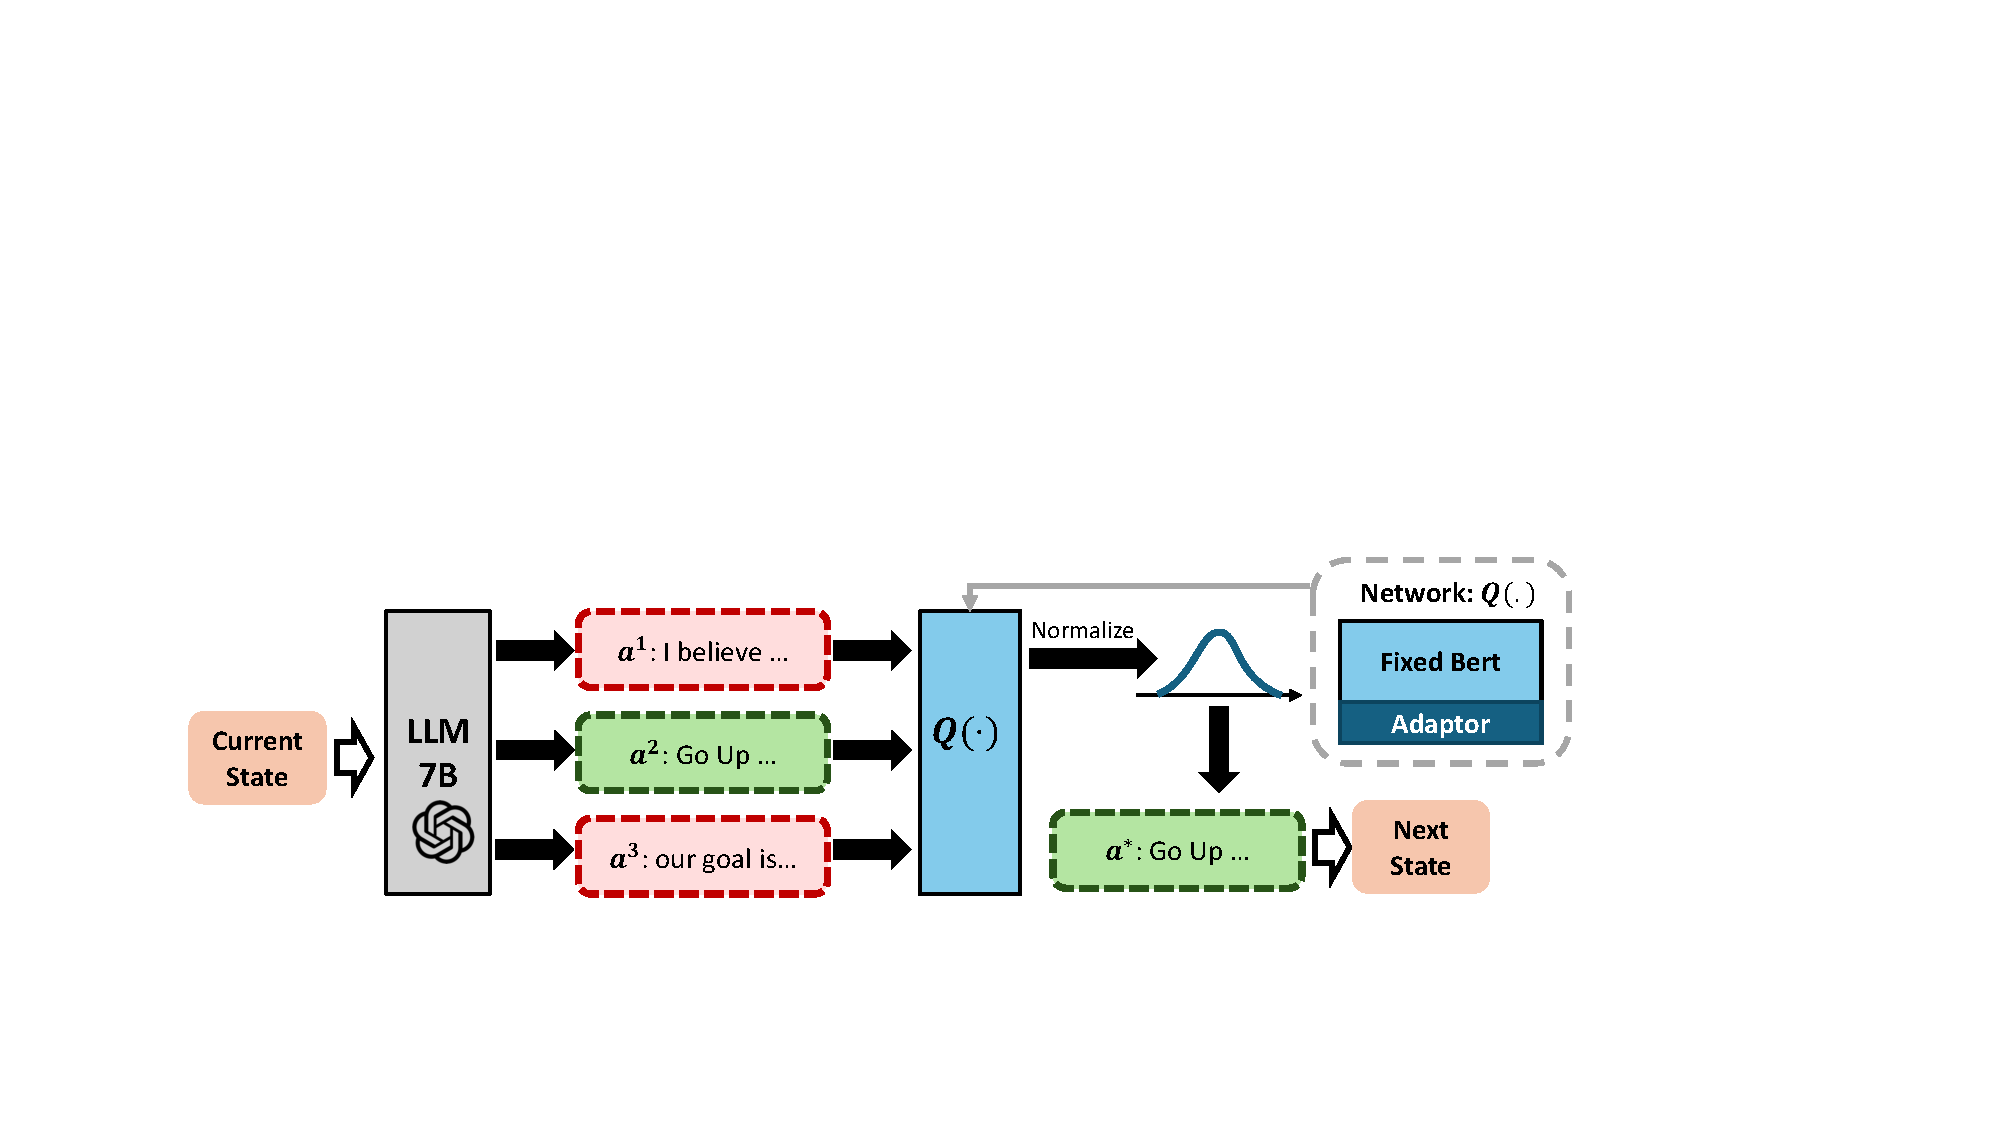
\includegraphics[width=\linewidth]{fig/Presentationfig.pdf}%framework
    \caption{An illustration of the process of approximate sampling from the intractable posterior: $ q(a | s, \mathcal{O} = 1) \propto p(\mathcal{O}=1|a,s_t)p_\text{LLM}(a|s_t)$, implemented by reweighting the action prior proposals according to $Q$-values, which act as likelihood estimates. In our experiments, the $Q$ function adopts BERT to encode textual state-action pairs and output a scalar value through an adaptor network.
% {Haitham: Please find this figure. Please write equations in Latex.}
 }
    \label{fig:sampling}
\end{figure}

% \begin{figure}
%     \centering    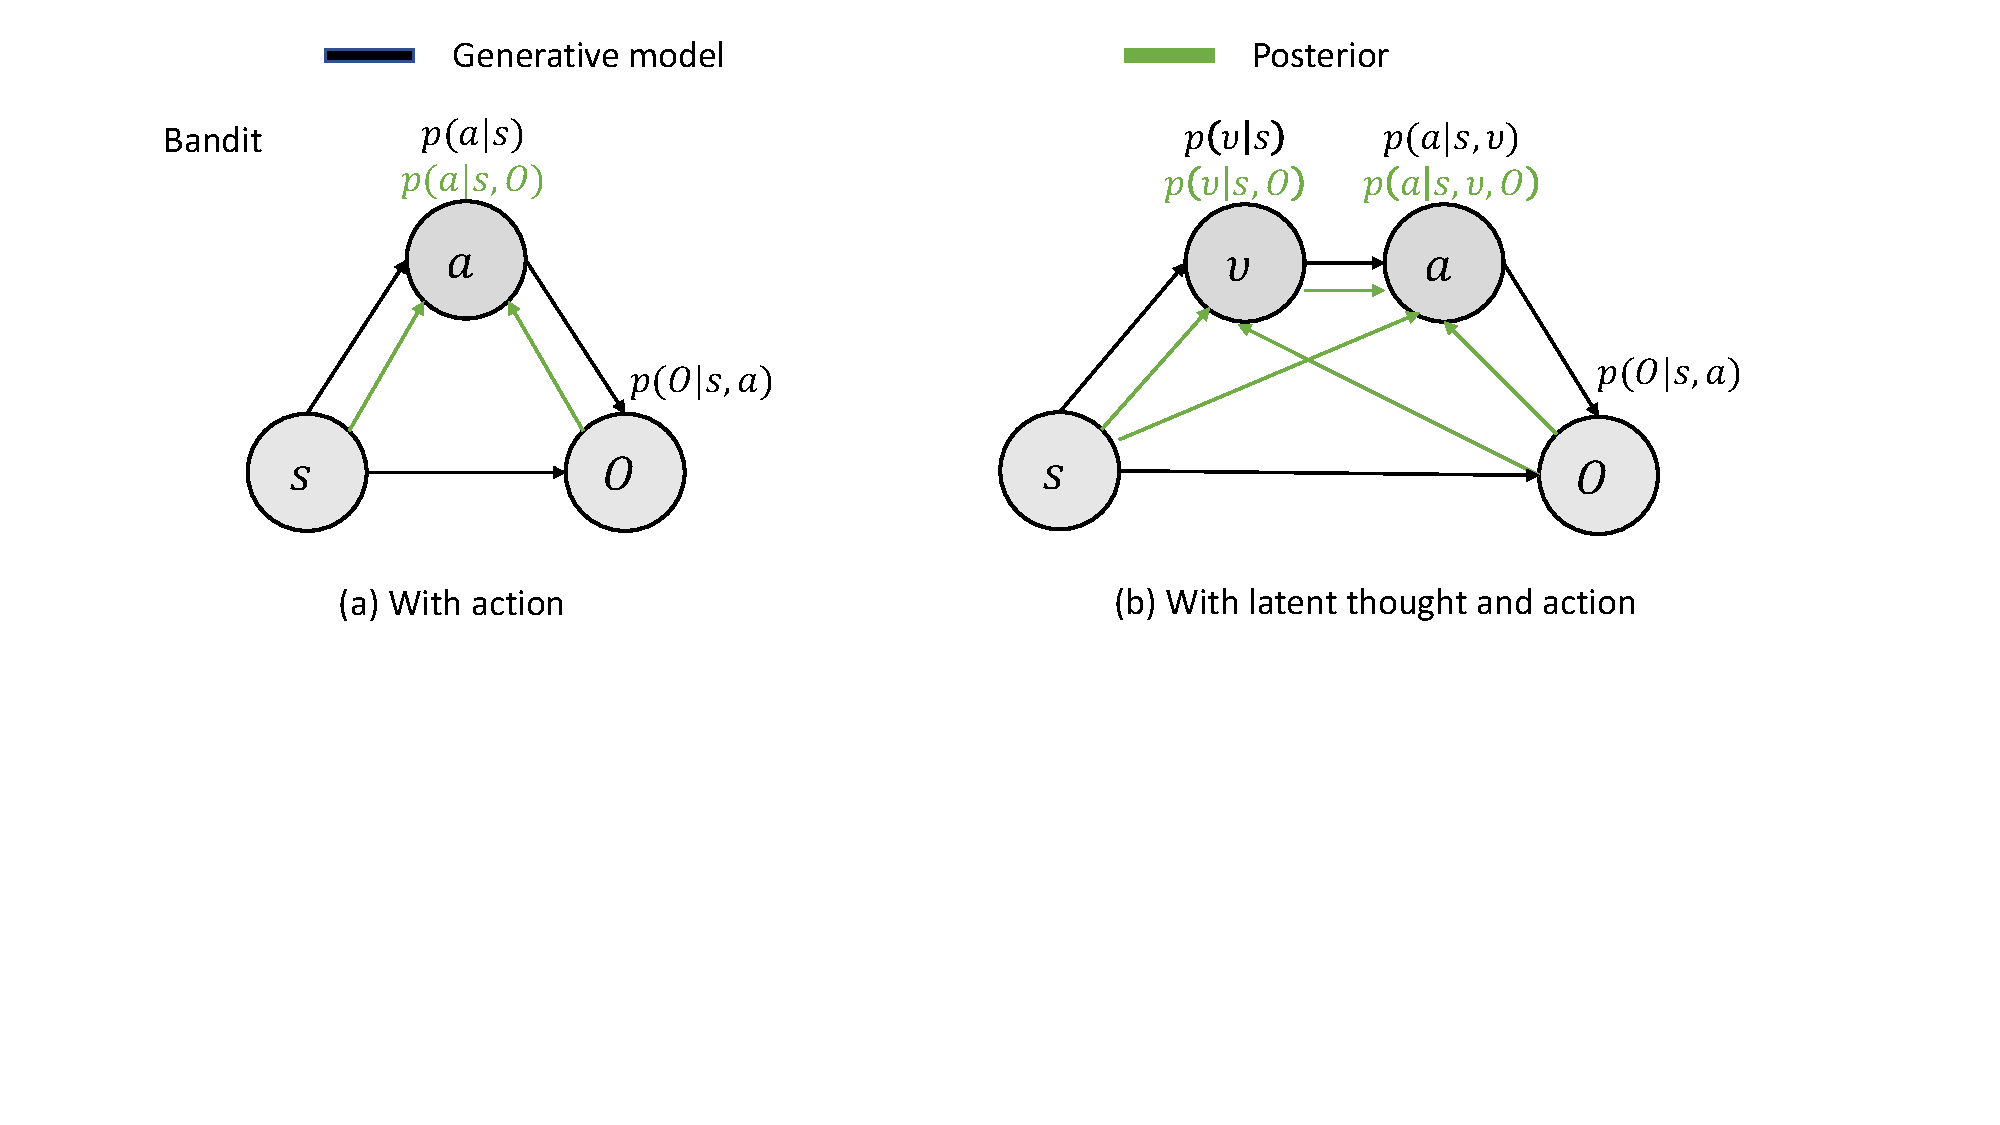
\includegraphics[width=0.9\linewidth]{fig/bandit_posterior.pdf}
%     \caption{The graphic model illustrates the generative and the desired \textcolor{green}{posterior} distribution on multi-armed bandit. (a) The situation of directly estimating the action $a$. (b) The situation of estimating the action $a$ via a latent thought $\upsilon$.
%     }
%     \label{fig:bandit_posterior}
% \end{figure}

% \begin{figure}
%     \centering
%     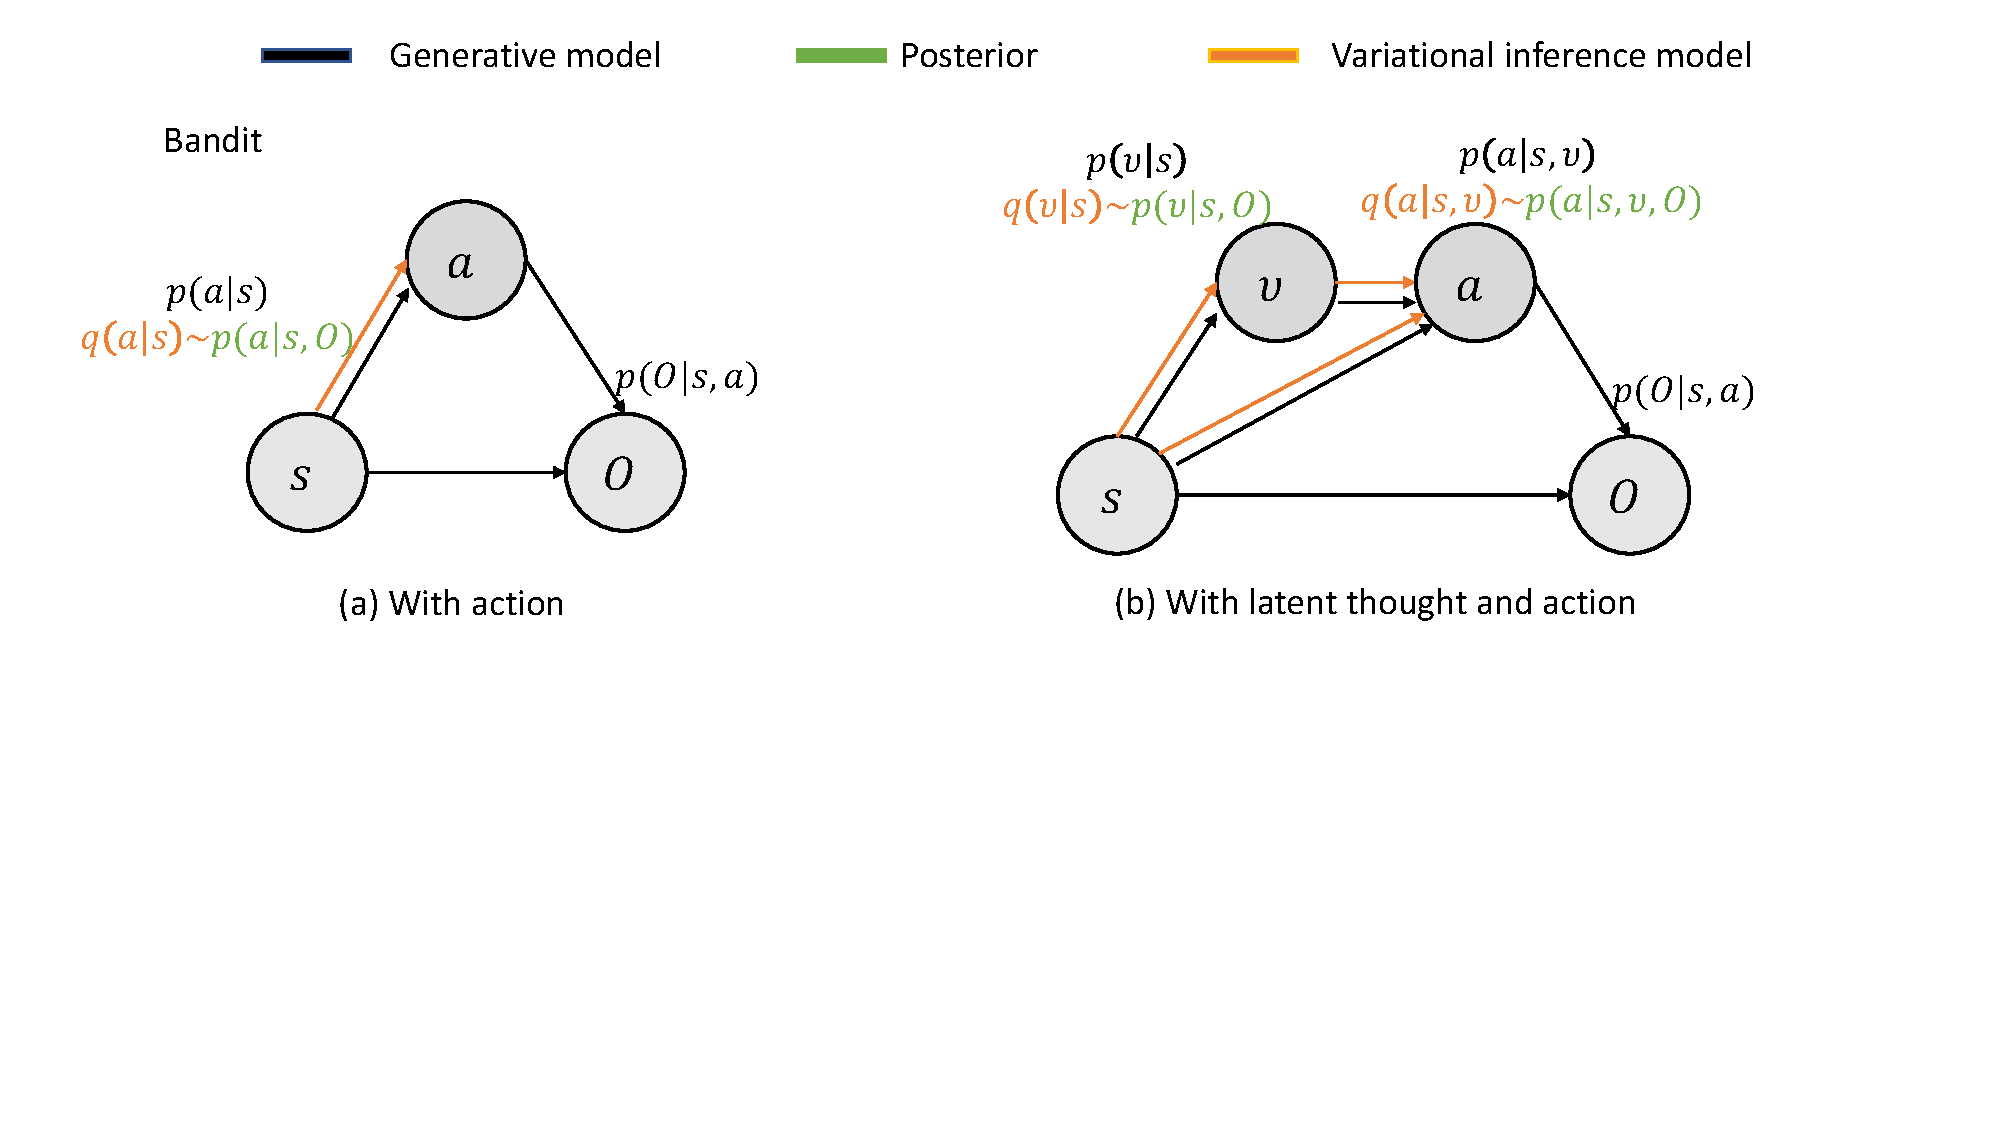
\includegraphics[width=0.9\linewidth]{fig/bandit_inference.pdf}
%     \caption{The graphic model illustrates the generative and the \textcolor{orange}{variational inference} to \textcolor{green}{true posterior} distribution on multi-armed bandit. (a) The situation of directly estimating the action $a$. (b) The situation of estimating the action $a$ via a latent thought $\upsilon$.}
%     \label{fig:bandit_inference}
% \end{figure}
% \begin{figure}[htbp]
%     \centering
%     % \rule{4cm}{4cm}
%     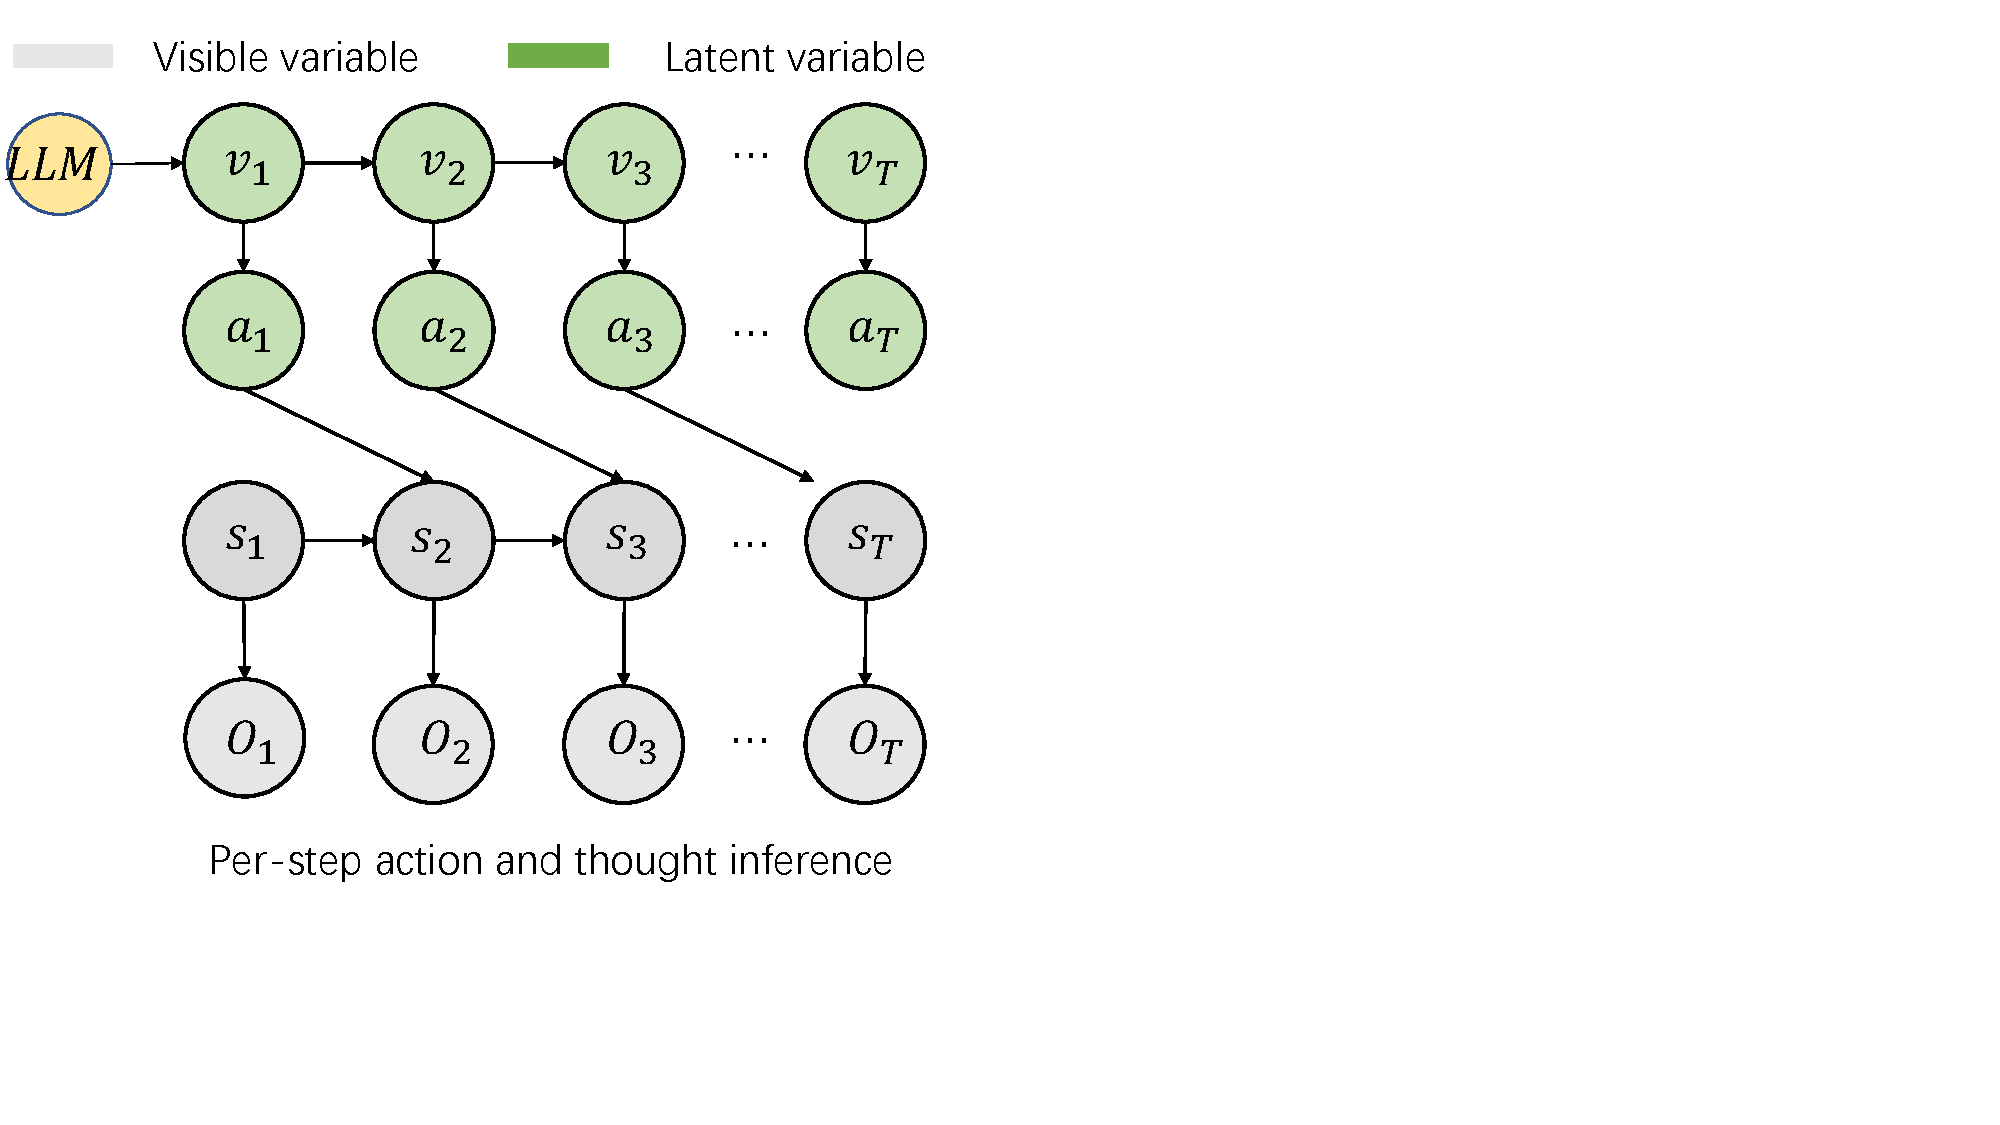
\includegraphics[width=0.5\linewidth]{fig/mtpformdp.pdf}
%     \caption{Graphic model of MDP graph with LLM thought}
%     \label{fig:mtpformdp}
% \end{figure}
% In this section, we describe how to solve the MTP. Specifically, we view the thought and action as latent variables and use the control as inference method to estimate the posterior of LLM and the posterior action policy for achieving optimality.

%\subsection{Control as Inference}
% \paragraph{Notation} We first list the mentioned notations for readers' convenience.  
% \newline
% $p_\mathcal{M}$: A LLM generative model. 
% $\bullet$ $p_\mathcal{M}(\upsilon|s)$: The thought generation policy based on a LLM $\mathcal{M}$. Or called the prior distribution over thoughts. This is a fixed prior. 
% $\bullet$ $p_\mathcal{M}(a|s)$: The action generation policy condition on state. 
% $\bullet$ $p_\mathcal{M}(a|s,\upsilon)$: The action generation policy condition on state and thought. 

% % $\bullet$ $\pi(a|s,\upsilon)$: The action policy.

% % $\bullet$ $p_\mathcal{M,\pi}$: The generative model with the thought policy $p_\mathcal{M}$ and action policy $\pi$.

% $\bullet$ $\mathcal{O}$: A random variable about the environment optimality 

% $\bullet$ $p_\mathcal{M}(a|s,\opt=1)$ The true poterior distrubion under the optimality variational condition. Or call $p(a|s,\opt=1)$ for simplity.

% $\bullet$ $q(a|s)$ the variational approximate of the posterior distribution over actions. 

% \paragraph{Notation} We first list the mentioned notations for readers' convenience.  

% $p_\mathcal{M}$: A LLM-based generative model. 

% $\bullet$ $p_\mathcal{M}(\upsilon|s)$: The thought generation policy based on an LLM $\mathcal{M}$, or called the prior distribution over thoughts. This is a fixed prior. 

% $\bullet$ $p_\mathcal{M}(a|s)$: The action generation policy conditioned on state. 

% $\bullet$ $p_\mathcal{M}(a|s,\upsilon)$: The action generation policy conditioned on state and thought. 

% $\bullet$ $\mathcal{O}$: A random variable about the environment optimality. 

% $\bullet$ $p_\mathcal{M}(a|s,\opt=1)$: The true posterior distribution under the optimality condition, or called $p(a|s,\opt=1)$ for simplicity.

% $\bullet$ $q(a|s)$: The variational approximation of the true posterior distribution $p_\mathcal{M}(a|s,\opt=1)$.
Since the optimal posterior distribution over trajectory $\tau$ can be factorized into step-wise posterior described as: $p(\tau|\mathcal{O}=1)\propto p(s_0)\prod_t p(a_t|s_t, \mathcal{O}=1)P(s_t|s_{t-1},a_{t-1})$, the learning procedure can be divided into two stages, modeling and inference of step-wise posterior $p(a|s_t, \mathcal{O}=1)$. The modeling stage will point out and decompose the desirable distribution into more solvable probabilistic terms. The inference stage will give the desirable outputs using sampling-based techniques \citep{korbak2022rl}.

% The learning procedure of $p(a|s_t, \mathcal{O}=1)$ can be divided into two stages, modeling and inference \citep{korbak2022rl}. The modeling stage will point out and decompose the desirable distribution into more solvable probabilistic terms. The inference stage will give the desirable outputs using sampling-based techniques.


% When attempting to incorporate LLMs into solving an MDP, the main objective is to find the posterior distribution over trajectories consistent with reaching the goal. This can be formally written as: $p(\tau|\mathcal{O}=1)\propto p(s_0)\prod_t p(a_t|s_t, \mathcal{O}=1)P(s_t|s_{t-1},a_{t-1})$. The primary challenge is learning the posterior distribution over actions $p(a|s_t, \mathcal{O}=1)$, {and we chose to sample directly from it}. 
%, and the posterior action policy can be transferred into: $p(a_t|s_t, \mathcal{O}=1)\propto p(\mathcal{O}=1|a_t,s_t)p(a_t|s_t)$ via the Bayes rule, which is a combination of the likelihood $p(\mathcal{O}=1|a,s)$ and the prior $p(a|s)$. Different from the optimality likelihood estimation in MAB, we assume the optimality likelihood as: $p(\mathcal{O}=1|a_t,s_t)\propto \exp(\sum_t r_t)$ following the generative model $p$, which is similar to the concept of the Q-function in reinforcement learning. In practice, we can use MCTS or TD-learning to estimate the optimality likelihood $p(\mathcal{O}=1|s_t,a_t)$.

%\yan{Whats the point of having this paragraph?}Instead of using a variational inference approach to learn a parametric action policy to approximate the action posterior, we apply probabilistic inference tools to achieve sampling from the intractable posterior. 
% The posterior inference can be divided into two stages, modeling and inference \citep{korbak2022rl}. The modeling stage will point out and decompose the desirable distribution into more solvable probabilistic terms. The inference stage will give the desirable outputs using sampling-based techniques.
\paragraph{Posterior Modeling}
We first use Bayes' rule to translate the intricate posterior into accessible terms:  
\begin{equation}
p(a|s_t, \mathcal{O}=1) =\frac{p(\mathcal{O}=1|a,s_t)p(a|s_t)}{p(\mathcal{O}=1|s_t)}\propto p(\mathcal{O}=1|a,s_t)p(a|s_t),
\end{equation}
which is a combination of the likelihood $p(\mathcal{O}=1|a,s_t)$ and the prior $p(a|s_t)$. Here, we use the LLM as the prior action distribution $p(a|s_t)\leftarrow p_\text{LLM}(a|s_t)$. %The graphical schematic of the generative model and the posterior distribution is shown in \fig \ref{fig:bandit_posterior} (a). 
Recall that the optimality likelihood in MDPs is given by: $ p(\mathcal{O}=1|a, s_t) \propto \exp\left(\sum_{i=t}  \gamma^{i-t}r_i\right) $, which corresponds to whether the goal state is achieved, similar to the concept of the Q function $Q(s_t,a)$ in RL. In practice, methods such as MCTS or TD-learning can estimate the optimality likelihood $p(\mathcal{O}=1|s_t, a)$ %\yan{Lack of motivation why we use RL. In appendix I have discussed Control as Inference where they link sampling from a posterior to soft Q-learning, we can take advantage of that?}.
% \paragraph{Token-level posterior inference} Suppose the action is a sentence consist of $k$ tokens: $a=a_1 a_2 \cdots a_k$, then we have          
% $$p(a|s,\mathcal{O}=1)=\prod_{i=1}^k p(a_i|s,a_{1\cdots i-1},\mathcal{O}=1).$$
% The token-by-token generation posterior can be factorized into:
% $$p(a_i|s,a_{1\cdots i-1},\mathcal{O}=1)=\frac{p(a_i|s,a_{1\cdots i-1})p(\mathcal{O}=1|s,a_{1 \cdots i})}{p(\mathcal{O}=1|s,a_{1\cdots i-1})}\propto p(a_i|s,a_{1\cdots i-1})p(\mathcal{O}=1|s,a_{1 \cdots i})$$
% \subsection{Sampling from intricate posterior distribution}
% \citep{hu2023amortizing} finetunes an LLM to amortize sampling from an intractable posterior distribution via the GflowNet objective. It's a variational inference approach that trains a parametric function to approximate the posterior. In this work, we use the sampling-based method at decoder time to achieve sampling from the posterior but do not need to finetune LLMs.  Decoder time sampling approaches include MCMC, Rejection Sampling, and Gibbs sampling. We discuss these well-established sampling approaches below:
% \paragraph{Directly approximate the posterior}
% If we learn a Q network with $(s,a_{1\cdots n-1})$ as input, and output a $|\mathcal{V}|$-dimensional vector, and the $i-th$ dimension indicates the Q vaule of $(s,a_{1\cdots n-1}\cup x_i)$ where $x_i$ is the $i$-th token in the vacabulary $\mathcal{V}$.

% Assume we have accessed the likelihood estimation $p(\mathcal{O}=1|s,a_{1\cdots i})$, then for each action generation step $i$, the $i$-th token is sampled by:
% \begin{equation}
%     a_i = \arg\max_x p(x|s,a_{1\cdots{i-1}})p(\mathcal{O}=1|s,a_{1\cdots i-1},x),
% \end{equation}
% where $x$ represents a token. 
\paragraph{Action Inference} %\yan{Also lack of motivation why we do action inference in this way. In appendix I have said that Levine discuss link to soft-q learning and he also offer a softmax formation for action inference which is exactly what we are talking about here. I have also discussed in the appendix the motivation of performing soft-Q learning over action subspace created by LLM prior.}
%\paragraph{Inference Policy Implementation Details}
Having described the posterior as a product between LLM prior $p_{LLM}(a|s_t)$ and estimate $Q$ function $ Q^\theta(s_t, a) $, we can implement the inference from the posterior distribution $p(a|s_t,\mathcal{O}=1)$ by following these steps:
\begin{itemize}
    \item Sample actions based on the prior policy $p_\text{LLM}$: Obtain $k$ action candidates for the current state $s_t$, denoted as: $\mathcal{C}^k(s_t)=\{a_1,a_2,\cdots,a_k\}$, where $a_i \sim p_\text{LLM}(a|s_t)$.
    \item Choose the next action from the candidates based on the estimated Q-values: Select an action $a^*$ according to the softmax probability distribution over the estimated Q-values. Specifically, $a^* \sim \operatorname{softmax}( Q^\theta(s_t, a_1)/\alpha,  Q^\theta(s_t, a_2)/\alpha, \dots, Q^\theta(s_t, a_k)/\alpha)$, where $\alpha$ is a hyper-parameter.
\end{itemize}
This sampling strategy is illustrated in \fig \ref{fig:sampling}, where the action candidates are reweighted based on the Q-values. 
%\paragraph{Connection between variational inference and posterior sampling} Denoting the above sampling strategy as following a distribution $q$, the following proposition shows that the posterior inference strategy is closely related to the variational inference solution of \eq \ref{variation} in expectation.
\begin{restatable}{props}{propsa}
\label{proposition}
Denote that the above sampling strategy indeed follows a distribution of $q$. When $k\rightarrow \infty$, we have:
\begin{equation}
\begin{aligned}
    \lim_{k\rightarrow\infty} q(a|s_t)&=  p_\text{LLM}(a|s_t){\exp( Q^\theta(s,a)/\alpha)}/{\mathbb{E}_{a_j \sim p_\text{LLM}(\cdot|s)} \exp( Q^\theta(s,a_j)/\alpha)}
\end{aligned}
\end{equation}
The limiting policy corresponds to the policy that optimizes the Q-values with a KL regularizer:
\begin{equation}
\begin{aligned}
        \lim_{k\rightarrow\infty} q(\cdot|s_t)&= \arg\max _\pi \mathbb{E}_{\pi(a|s_t)} [Q^\theta(s_t,a)]-\alpha \text{KL}\left(\pi(\cdot|s_t)\|p_\text{LLM}(\cdot|s_t)\right)
\end{aligned}
\end{equation}
Then, the posterior sampling strategy is highly related to the solution of variational inference as shown in \eq \ref{variation}. %when the $Q^\theta$ values is estimated following the optimal $\pi*$ such that $\pi^*=\arg\max_\pi \sum_t \gamma^t r_t-\alpha \text{KL}(\pi(\cdot|s_t)\|p_\text{LLM}(\cdot|s_t)))$.
Proof. Please see the appendix. %\yan{\st{When convergence, $ Q^\theta(s_t,a)\propto \sum_t \gamma^{i-t}r_i$.}}
\end{restatable}
% \paragraph{Token level Rejection Sampling}
% Since mapping the $(s,a_{1\cdots n-1})$ into $|\mathcal{V}|$ scalars with very sparse supervision signal and the action space is huge. Thus, we alternative learn a Q-network that directly map the sentence embedding of $(s,a_{1\cdots n-1})$ into one scales which indicates the Q-value of $(s,a_{1\cdots n-1})$, while it  approximates the likelihood $p(\mathcal{O}=1|s,a_{1\cdots n-1})$.
% ∙\bullet q(τ)q(\tau): An auxiliary distribution over trajectory consistent with the optimality condition. 

% ∙\bullet q(υ|s)q(\upsilon|s) (q(υ|s,O)q(\upsilon|s,\mathcal{O})): An auxiliary distribution over thoughts consistent with the optimality condition. Or called the posterior conditioned on the optimality.

% ∙\bullet q(a|s,υ)q(a|s,\upsilon) the variational approximate of the posterior distribution over actions. 


% Suppose the $q(\upsilon|s)$ is also served by LLM customized for a specific decision process. We can either finetune an LLM to adapt to the specific task or use a small model to distill the outputs of LLMs.

% To convenient the learning process the LLM posterior and avoid expensive fine-tuning on LLMs for a specific task, we can use probabilistic inference techniques like EM to estimate the posterior distribution. The probabilistic inference method have been used for decision-making tasks, taking the classical MPO \citep{abdolmaleki2018maximum} as an example that treats the policy optimization as a maximum posterior distribution problem. Firstly, we define the optimality like MPO as $p(O=1|\tau)\propto exp(\sum_t r_t/\alpha)$. In the field of CAI, the objective function is to optimize the distribution over trajectories $\tau$, such that maximizing the probability of reaching the optimality, formally written as $\max\mathbb{E}_{p(\tau)} [p(\mathcal{O}=1|\tau)]$.
\iffalse
\subsection{Probabilistic Inference with LLM Prior on Multi-Armed Bandit}

The variational distribution over actions is expected to approximate the true posterior distribution of the generative model conditioned on optimality. The graphic illustration of the generative model and the variational approximation is depicted in \fig \ref{fig:bandit_inference}(a). The objective function of the variational approximation is to minimize the below KL-divergence:
\begin{equation}
\begin{aligned}
    &\text{KL}(q(a|s)\|p_{\mathcal{M}}(a|s,O=1))\\
    &=-\mathbb{E}_{q(a|s)} \log \frac{p_{\mathcal{M}}(a|s,O=1)}{q(a|s)}\\
    &=\mathbb{E}_{q(a|s)} \log q(a|s)-\mathbb{E}_{q(a|s)}\log p_{\mathcal{M}}(a|s,O=1)\\
    &=\mathbb{E}_{q(a|s)} \log q(a|s)-\mathbb{E}_{q(a|s)}\log\frac{p_{\mathcal{M}}(a,O=1|s)}{p_{\mathcal{M}}(O=1|s)}\\
    %&=\mathbb{E}_{q(\upsilon,a|s)}\left[\log q(\upsilon,a|s)-\log p_{\mathcal{M},\pi}(\upsilon,a,O=1|s)+\log{p_{\mathcal{M},\pi}(O=1|s)}\right]\\
    &=\mathbb{E}_{q(a|s)}\left[\log q(a|s)-\log p_{\mathcal{M}}(a,O=1|s)\right]+\log{p_{\mathcal{M}}(O=1|s)},\\    
\end{aligned}
\end{equation}
Due to the KL divergence always being greater than $0$, and the term $\log{p_{\mathcal{M}}(\mathcal{O}=1|s)}$ being irrelevant to the approximated posterior $q(a|s)$, we can alternatively minimize the following objective function:
\begin{equation}
\label{"state_obj"}
\begin{aligned}
        & \mathbb{E}_{q(a|s)}\left[\log p_{\mathcal{M}}(a,O=1|s)-\log q(a|s)\right]\\
        % &\stackrel{(1)}{=}\mathbb{E}_{q(\upsilon|s)}[\log p(\mathcal{O}=1|s)]-\mathbb{E}_{q(\upsilon|s)}\left[KL(q(a|\upsilon,s)\|p(a|\upsilon,s))\right]-KL(q(\upsilon|s)\|p(\upsilon|s,\mathcal{O}=1)) \\
        &\stackrel{(1)}{=}\mathbb{E}_{q(a|s)}[\log p_{\mathcal{M}}(\mathcal{O}=1|s,a)]-KL(q(a|s)\|p_\mathcal{M}(a|s)) \\
        %&=\log p_{\mathcal{M},\pi}(\mathcal{O}=1|s)-KL(q(a|s)\|p_\mathcal{M}(a|s))\\
        &=\mathcal{J}(q)
    %     &=\mathbb{E}_{q(\upsilon,a|s)}\left[\log p_{\mathcal{M},\pi}(O=1|s,\upsilon)+\log p_\mathcal{M}(\upsilon|s)-\log q(\upsilon|s)\right]\\        &=\mathbb{E}_{s\sim\rho}\left[\mathbb{E}_{q(\upsilon|s)}\left[\log p_{\mathcal{M},\pi}(O=1|s,\upsilon)\right]\right]-\text{KL}( q(\upsilon|s)\| p_\mathcal{M}(\upsilon|s))\\
    %     &=\mathbb{E}_{s\sim \rho}\left[\mathbb{E}_{q(\upsilon|s)}\left[\log \sum_a p_{\mathcal{M},\pi}(O=1|s,\upsilon,a)\pi(a|s,\upsilon)\right]\right]-\text{KL}( q(\upsilon|s)\| p_\mathcal{M}(\upsilon|s))\\
    %     &=\mathbb{E}_{s\sim \rho}\left[\mathbb{E}_{q(\upsilon|s)}\left[\log V_{\mathcal{M},\pi}(s,\upsilon)/\alpha\right]-\text{KL}( q(\upsilon|s)\| p_\mathcal{M}(\upsilon|s))\right]\\
\end{aligned}
\end{equation}
%\yanxue{assume the optimality is only related to s}
% Where the equation (1) holds due to the decomposition of $p_{\mathcal{M},\pi}(\upsilon,a,\mathcal{O}=1|s)=p(\mathcal{O}=1|s)p(a|\upsilon,s)p(\upsilon|s,\mathcal{O}=1)$ with $a$ is independent to the optimality? 
The equation $(1)$ holds due to the decomposition $p_{\mathcal{M}}(a,\mathcal{O}=1|s)=p(a|s)p_{\mathcal{M}}(\mathcal{O}=1|s,a)$. It is straightforward to observe that if we set the variational posterior as $q(a|s)\propto p_{\mathcal{M}}(\mathcal{O}=1|s,a)p_\mathcal{M}(a|s)$, then the objective function $\mathcal{J}(q)$ is reduced to a constant term $\log \sum_a \log p_\mathcal{M}(\mathcal{O}=1|s,a)p_\mathcal{M}(a|s)$.

In practice, we assume that conditional optimality in the multi-armed bandit is related to the reward $p_\mathcal{M}(\mathcal{O}=1|s,a)\propto r(s,a)$. Thus, we use historical rewards sampled from a stochastic and unknown true distribution to estimate the true reward, maybe averaged reward or UCB estimation. $p_\mathcal{M}$ represents a language model (LLM) prior, which is incorporated due to the possibility that it contains task-solving relevant knowledge obtained by pre-training on a large corpus.
\paragraph{Remarks}We explain the solution for the posterior over the action. Instead of using a variational approximation to the posterior, we directly apply Bayesian inference to the intractable posterior to estimate it. The optimal action policy in the multi-armed bandit problem can also be seen as learning a conditional policy $p(a|s, \mathcal{O}=1)$ conditioned on optimality. This conditional optimal policy is intractable, so we can use Bayes' rule to translate it to $$p(a|s, \mathcal{O}=1) \propto p(\mathcal{O}=1|a,s)p(a|s),$$ which is a combination of the likelihood $p(\mathcal{O}=1|a,s)$ and the prior $p(a|s)$. The graphic schematic of the generative model and the posterior distribution is shown in \fig \ref{fig:bandit_posterior} (a).
%=p(\upsilon|s)p(a|\upsilon,s)p(\mathcal{O}=1|s)$. The last equation holds due to the assumption of that the optimality is only related to $s$. 

%Due to the generative agent policy $\pi(a|\upsilon,s)$ being unknown, we first design an algorithm to estimate this policy so that it can meet the optimality as possible.

% Due to the unknown nature of the generative agent policy $\pi(a|\upsilon,s)$, we first develop an algorithm to estimate this policy to achieve optimality.
\fi

\section{Practical Implementation}\label{sec: implementation}
% Following the analysis in Sec. \ref{sec: method}, we use Bayesian inference tools to incorporate the LLM prior into decision-making. 
In this section, we introduce the practical implementation of posterior approximation within robust RL frameworks. We describe a policy-based RL method with an LLM prior to solve the variational inference problem. In the meantime, as discussed earlier, optimality likelihood estimation is critical for direct posterior inference and is positively associated with Q-values in the MDP setting. We consider Q-value estimation with an LLM prior for value-based RL in both online and offline settings. Finally, we propose three simple yet efficient RL algorithms: one policy-based RL algorithm and two Q-learning variants.
%, by incorporating the LLM prior into the exploration or optimization processes. 

We will first introduce the two Q-learning variants, which perform exploration and optimization within a narrowed yet reliable LLM prior action space, eliminating the need for fine-tuning the language model-based policy. Then, we will present a policy-based PPO variant that incorporates a KL loss with respect to the LLM prior. Detailed descriptions of classic Q-learning algorithms, DQN \cite{mnih2013playing} and CQL \cite{kumar2020conservative}, can be found in the Appendix.
%\subsection{Estimate Likelihood with LLM Prior}
 %Note that several studies for improving reasoning ability of LLMs can be derived as special cases of our posterior sampling framework. These works have investigated several likelihood estimation approaches, for example, \citep{feng2023alphazero,hao2023reasoning} use heuristic search-based planners or  \citep{yao2024tree, zhang2024can} let LLMs as evaluators. However, these estimation approaches often require a large number of interactive samples or meticulous human labor.
%In this work, 
%we opt to employ temporal difference learning \citep{tesauro1995temporal} as a computationally more efficient estimate of the optimality likelihood. 
%To avoid fine-tuning which is computationally expensive, we apply direct posterior sampling with a learned likelihood function and a fixed LLM as a probabilistic prior. Specifically, the LLM provides a narrowed yet reliable subset of the complete action space, where each action is reweighted by the likelihood function, and the executed action is sampled accordingly. For the learning of the likelihood function, we utilize value-based RL with TD learning to learn Q-values which estimate optimality. We apply this idea to improve sample efficiency in online RL settings, and simplify optimization space in offline RL settings.
\subsection{Online Value-Based RL with LLM prior} 
%DQN \citep{mnih2013playing} is a widely used value-based RL method for training a Q-network, denoted as $Q_\theta$. It alternates between exploring new data using the latest Q-function and updating the Q-function by applying the Bellman optimal operator on the replay buffer $\mathcal{D}$, which stores previously collected data.
\label{sec: online_value_rl}
The Q-value estimation is based on DQN \citep{mnih2013playing}, a widely used value-based RL method, under the online setting. Unlike traditional DQN, which performs exploration and Bellman updates over the full action space $\mathcal{A}$, we propose a variant with an LLM prior, referred to as DQN-Prior. This variant limits these processes to the prior action space $\mathcal{C}^k \subseteq \mathcal{A}$, which is sampled from $p_\text{LLM}$. This prior action space represents a reduced and more rational subspace where clearly irrelevant actions may be filtered out in advance. Specifically, DQN-Prior alternates between the following steps:
\paragraph{Exploration} 
Roll out new episodes using the posterior inference strategy as described in Sec. \ref{posterior_infer}, specifically:
\begin{itemize}
    \item For a state $s_t$, sample the action prior space $\mathcal{C}^k(s_t)=\{a_1,a_2,\cdots,a_k\}, a_i \sim p_\text{LLM}(a|s_t)$. 
    \item Then sample the action $a_t\sim \operatorname{softmax}\left({Q^\theta(s_t,a_1)/\alpha},\cdots,{Q^\theta(s_t,a_k)/\alpha}\right)$. 
    \item Apply the action $a_t$ to the environment, and obtain the next state $s_{t+1}\sim P(\cdot|s_t,a_t)$. 
    \item Add the tuple to the reply buffer: $\mathcal{D}=\mathcal{D}\bigcup (s_t,a_t,s_{t+1})$. 
\end{itemize}
\paragraph{Q-function Update} After expanding the replay buffer, we use TD-learning to update the Q-network. The loss function for the $i$-th iteration is given as:
\begin{equation}
\label{dqn-prior}
\mathcal{L}_i(\theta)=\mathbb{E}_{(s,a,s^\prime)\sim \mathcal{D}}\left[(Q^{\theta_i}(s,a)-y_i)^2\right],
\end{equation}
where $y_i=\mathcal{B}^*Q^{\theta_{i-1}}(s,a)=r(s,a)+\gamma \max_{\textcolor{red}{a^\prime\in \mathcal{C}^k(s^\prime)}} Q^{\theta_{i-1}}(s^\prime,a^\prime)$.
Compared to traditional DQN, the DQN-Prior performs exploration and applies the Bellman optimal operator within the LLM prior action space, as highlighted in \textcolor{red}{red} in \eq \ref{dqn-prior}.

To represent the Q-network, we introduce an adapter on top of the LLM embeddings and fit the adapter's weights by minimizing the temporal difference loss. In our work, the LLM (i.e., BERT \citep{devlin2018bert}) is used to encode state and action pairs and is frozen during optimization, as illustrated in \fig  \ref{fig:sampling}. Therefore, we do not propagate any gradients through the LLM to avoid expensive computational overhead.

\subsection{Offline Value-Based RL with LLM Prior}
\label{sec: offline_value_rl}
%As analyzed previously, we have provided an efficient method for LLMs to solve SDM tasks while eliminating the need for fine-tuning. The critic process, i.e., the accurate estimation of Q-values, necessitates a large amount of data. During implementation, we can iteratively collect data online based on approximate posterior sampling and then refine the Q-value estimation accordingly. Thus, we can finally achieve desirable posterior estimation through this bootstrap process, utilizing the fixed LLM as the prior action distribution. However, despite avoiding the time and resource-intensive fine-tuning process, online exploration for data collection remains time-consuming, as it requires querying the LLM for each state.

%Therefore, this study also investigates the feasibility of using gradient-free LLM priors for accurate action posterior estimation solely based on offline datasets. 
This study also explores the feasibility of using gradient-free LLM priors for successful SDM based solely on offline datasets.
\citep{snelloffline} have explored the use of offline RL for language generation tasks based on the SFT LLM from offline datasets. This approach assumes the entire token vocabulary as the action space, where each action corresponds to a single token, resulting in a vast action space with tens of thousands of possible actions. In our work, we consider a discrete action space where each action is a short phrase consisting of several tokens. For the SDM tasks we address, the action space is significantly smaller, with fewer than a hundred possible actions. Additionally, by leveraging an action prior, we can first obtain a tidy sub-action space $\mathcal{C}^k$, thereby narrowing the optimization space. 

We apply this action prior within the CQL framework, a widely used offline RL approach, and refer to this variant as CQL-Prior. The loss function for the proposed CQL-Prior is given as:
\begin{equation}
\label{cql_loss}
\mathcal{L}_i(\theta)=\beta\mathbb{E}_{(s,a)\sim \mathcal{D}}\left[\log \sum_{\textcolor{red}{a^\prime\in \mathcal{C}^k(s)}} \exp(Q^{\theta_i}(s,a^\prime))-Q^{\theta_i}(s,a)\right]+\frac{1}{2}\mathbb{E}_{(s,a,s^\prime)\sim \mathcal{D}} \left[(Q^{\theta_i}(s,a)-y_i)^2\right],
\end{equation}
where $y_i=r(s,a)+\gamma \max_{\textcolor{red}{a^\prime\sim \mathcal{C}^k(s^\prime)}} Q^{\theta_{i-1}}(s^\prime,a^\prime)$ and $\beta$ is a hyper-parameter. The main difference from traditional CQL is that it restricts the overestimation of Q-values to the tidy action prior space and applies the Bellman optimal operator within this space, as highlighted in red.
\subsection{Policy-based RL with LLM Prior}
\label{sec: online_policy_rl}

We implement variational inference for MDPs with LLMs as action priors using a policy-based RL framework. Specifically, we build upon GFlan \citep{carta2023grounding}, let the Flan-T5 small model \citep{rae2021scaling} (with less than $1B$ parameters) as the action policy for leveraging pre-stored knowledge to solve complex SDMs and fine-tune it via Proximal Policy Optimization (PPO) \citep{schulman2017proximal}. Our variant, called GFlan-Prior, incorporates a KL regularizer into the PPO loss to optimize \eq \ref{variation}. During implementation, we sample $k=5$ examples from LLM prior distribution $p_\text{LLM}(a|s)$ to compute the approximated KL divergence.
Formally, for the $i$-th iteration, the policy $\pi_{\theta_i}$ is learned by optimizing:
\begin{equation}\label{ppo}\arg\max_\theta\mathbb{E}_{(s_t,a_t)\sim \pi_{\theta_{i-1}}}\text{CLIP}\left(\frac{\pi_\theta(a_t|s_t)}{\pi_{\theta_{i-1}}(a_t|s_t)}\right)\hat{A}_t+\gamma \mathcal{H}(\pi_\theta(\cdot|s_t))-\alpha\text{KL}[\pi_\theta(\cdot|s_t)\|\hat{p}_\text{LLM}(\cdot|s_t)],
\end{equation}
where $A_t$ is the estimated advantage, $\gamma$ is the hyperparameter that encourages exploration, and $\hat{p}_\text{LLM}(\cdot|s_t)$ is the discrete distribution constructed by $k$ action proposals from the LLM. ${\theta_{i-1}}$ represents the parameters of the action policy learned in the last iteration.
% \begin{figure}[htbp]
%     \centering
%     % \rule{4cm}{4cm}
%     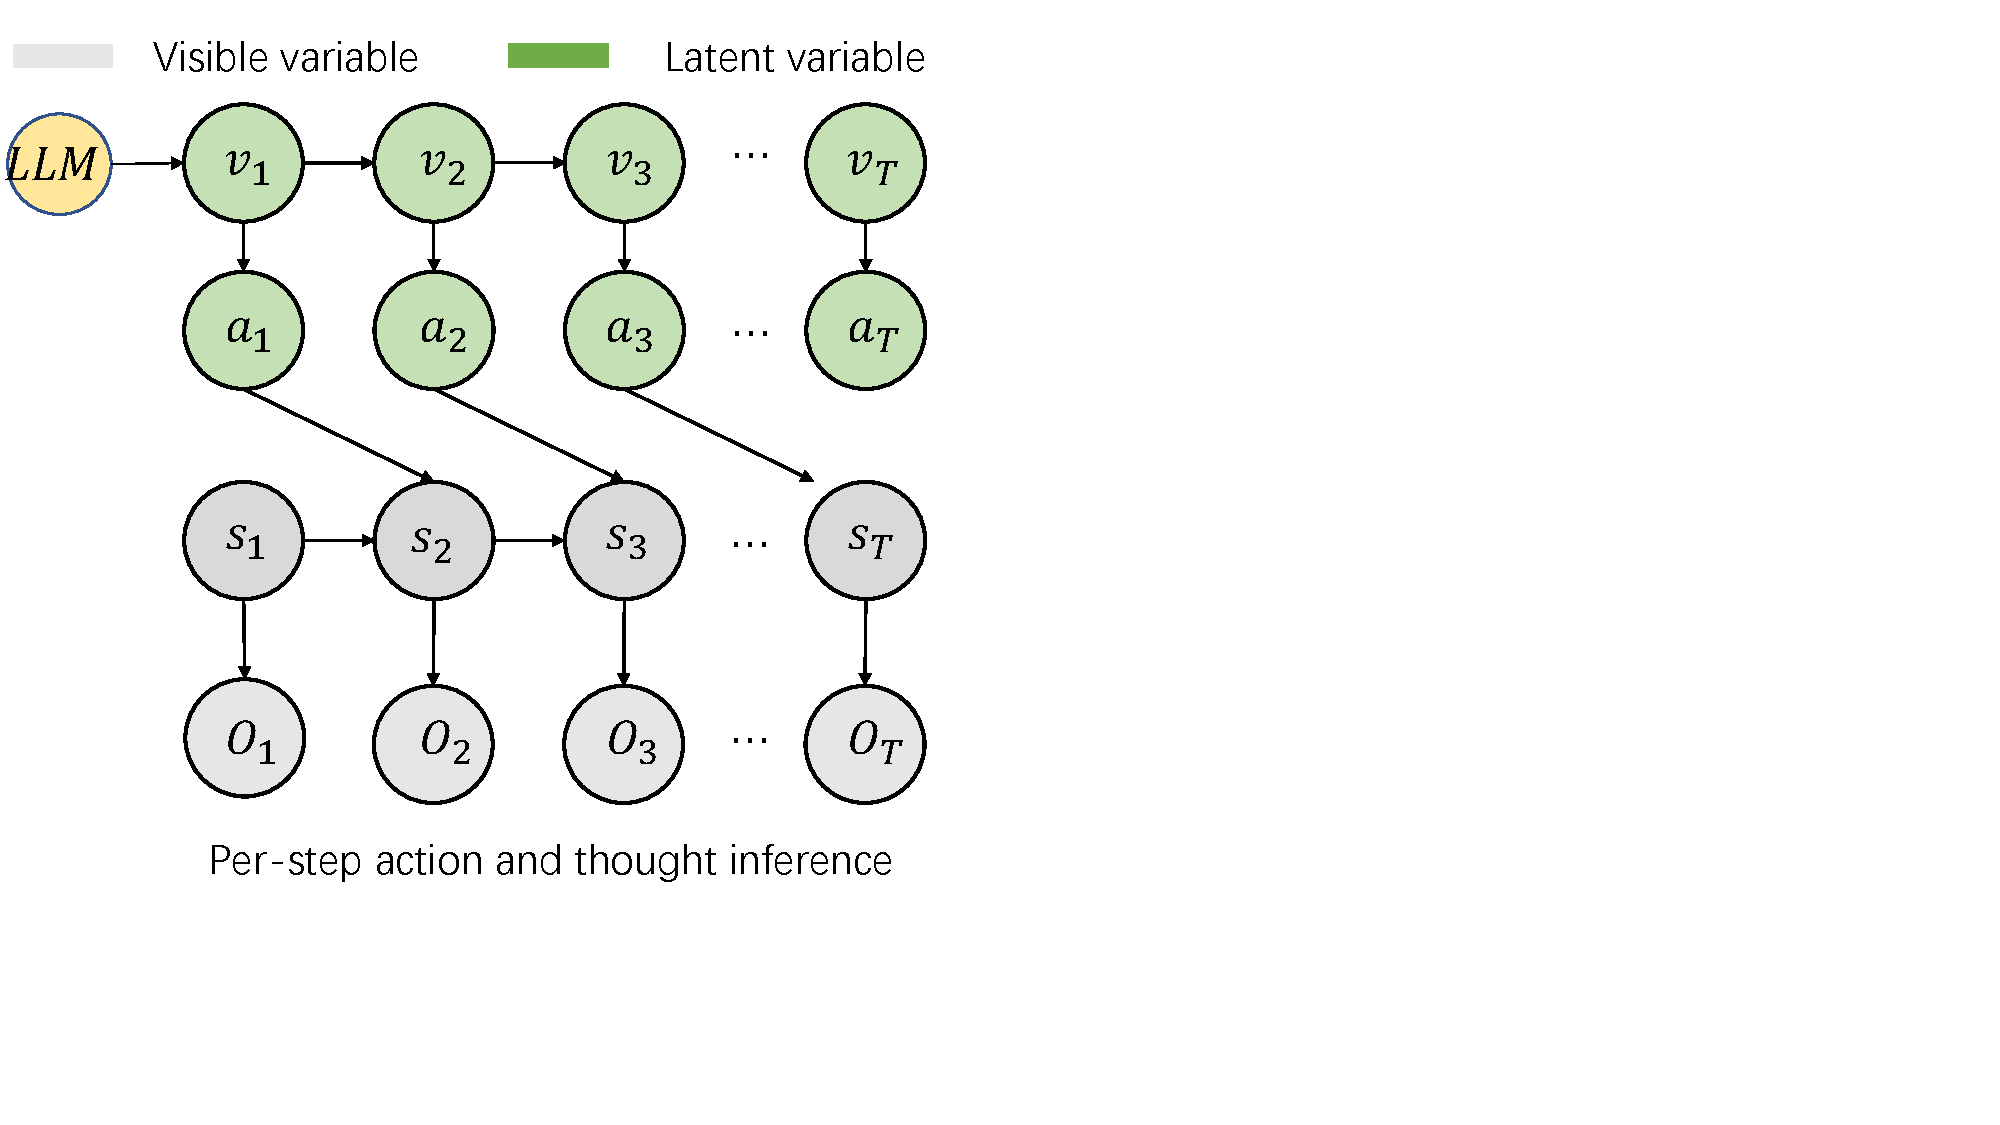
\includegraphics[width=0.5\linewidth]{fig/mtpformdp.pdf}
%     \caption{Graphic model of MDP graph with LLM thought}
%     \label{fig:mtpformdp}
% \end{figure}
% In this section, we describe how to solve the MTP. Specifically, we view the thought and action as latent variables and use the control as inference method to estimate the posterior of LLM and the posterior action policy for achieving optimality.
% \subsection{Q value training and optimal policy inference with LLM prior}





% \paragraph{Motivation of incorporating a CoT thought process} CoT reasoning have proved to show significant performance improvement in solving complicated decision making tasks such as ToT and RAP. Inspired by utilising further CoT reasoning during making decisions we introduce the model with CoT thought. The naive action policy with the form of $p_\mathcal{M}(a|s)$. Then we design a more complete version of the decision policy with latent thought $p_\mathcal{M}(a|s)=\sum_\upsilon p_\mathcal{M}(\upsilon|s)p_\mathcal{M}(a|\upsilon,s)$, where $p_\mathcal{M}$ is generative model served by LLMs.
\begin{figure*}[t!]
\centering
	  
\includegraphics[width=0.5 \linewidth]{fig/legendbaselineprior.pdf}\\
{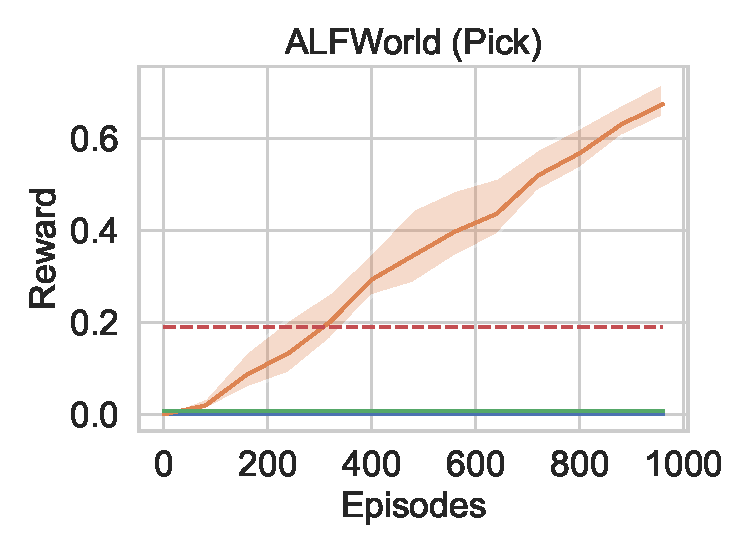
\includegraphics[width=0.30\linewidth ]{fig/train_curve_alf_pick.pdf}}
{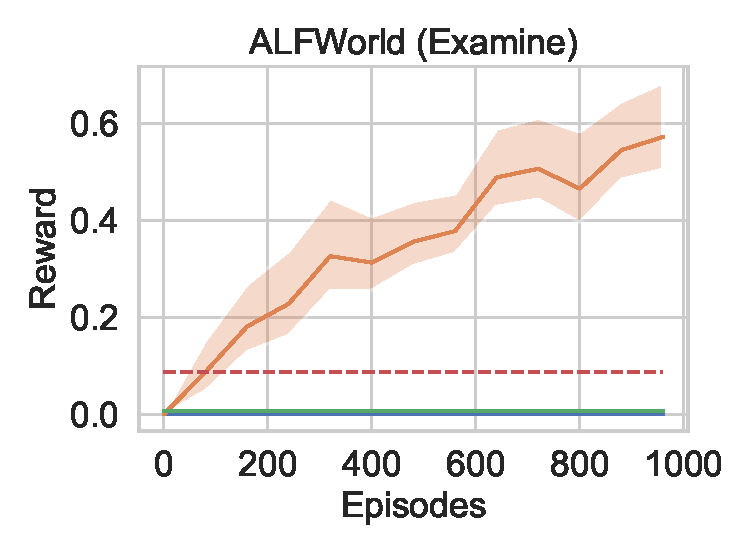
\includegraphics[width=0.30 \linewidth ]{fig/train_curve_alf_exam.pdf}}
    	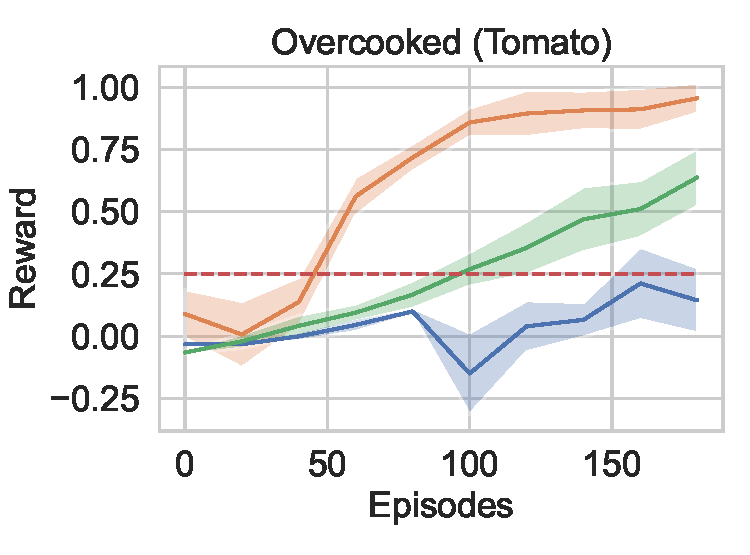
\includegraphics[width=0.30 \linewidth]{fig/train_curve_overcooked.pdf}
    {    
    %\label{fig:chainbar}    
    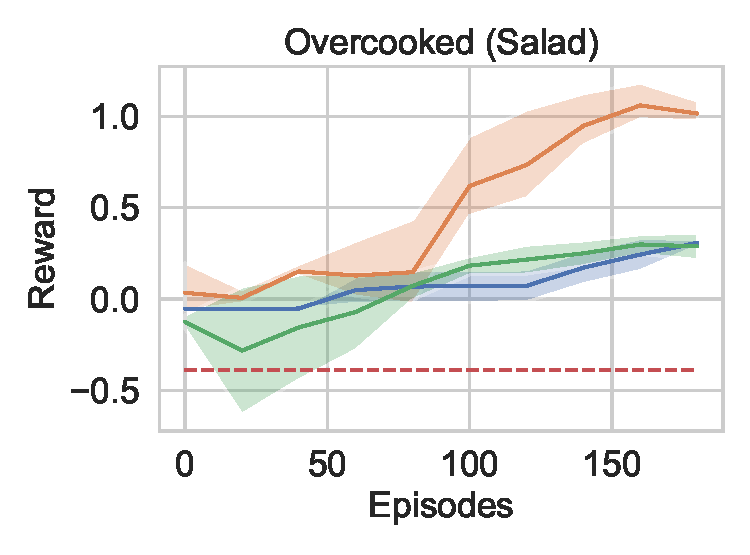
\includegraphics[width=0.30 \linewidth]{fig/train_curve_overcooked_lettuce.pdf}}
% \vspace{-1.0cm}
      % \vspace{-2.3em}
           {
 %\label{fig:chaintraining}
    	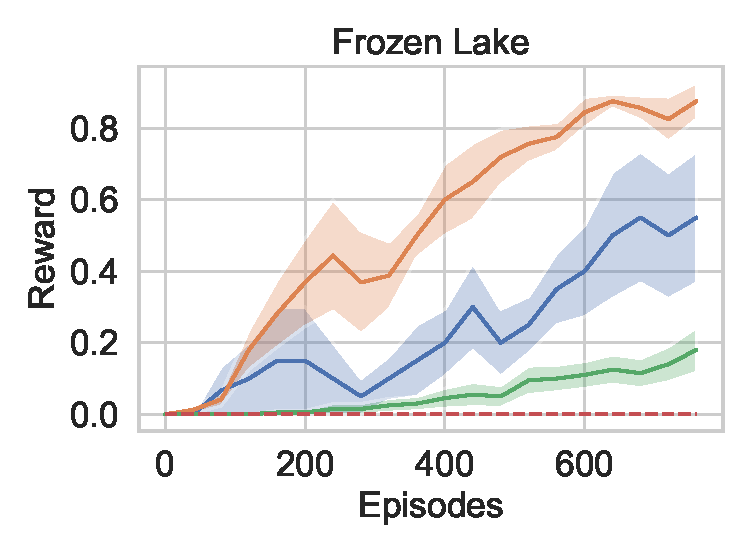
\includegraphics[width=0.30 \linewidth]{fig/train_curve_frozenlake.pdf}
    		}
     
     
   % \subfigure[(Tomato)]
 %\label{fig:chaintraining}
%\subfigure[]

%,height=2cm]
	%\subfigure[]
 {
 %\label{fig:chaintraining}
    		}
    
       % \subfigure[(Salad)]
        
    % {fig/overcooked_large_auc.pdf}
      %\vspace{-0.7em}
    \caption{{Results of comparison with online baselines. We plot the mean and standard error of the cumulative reward. For inference baselines, the reward is averaged over $20$ episodes. We plot the rewards averaged over the final third of the training processes for trainable baselines across five random seeds. %\textbf{Please make figures bigger. They are not readable. try to use trim from latex to see if it can help. If not we can split across multiple lines. }
    %We plot the mean and standard error of nomalized reward averaged over $5$ seeds for trainable baselines, and over $20$ episodes for GPT-3.5 baselines. For trainable baselines, we plot the normalized rewards, averaged over the latter part of the training process. The cumulative rewards are normalized within the range $[0, 1]$.
    %The Area Under the Curve (AUC) is calculated by averaging the normalized rewards from the latter part of the training process.
    %The cumulative rewards are normalized within the range $[0, 1]$, and the Area Under the Curve (AUC) is calculated by averaging the back part of the training process.%the entire training process. %We normalize the cumulative rewards within the range $[0,1]$ and calculate the Area Under the Curve (AUC) by averaging over the whole training process.
    }}% during training or inference.}}  %These results plot the a verage reward of episodes with $400$ timesteps. For each baseline, we train $5$ different models varying only over random seeds and. 
    %} 
\label{fig:baselinesdqn}
% \vspace{-1.0em}
\end{figure*}


\section{Experiments}
\label{sec: exp}

%In this work, we attempt to leverage the rich domain knowledge and strong reasoning abilities of LLMs to solve complex decision-making tasks. We view the powerful LLM as an action prior distribution and analyze, from a Bayesian inference perspective, how to incorporate LLM priors into the solving process of MDPs. 
In this section, we demonstrate the effectiveness of incorporating the LLM prior into the RL framework, including both policy-based and value-based algorithms in online and offline settings. LLM priors are used to reduce the exploration and optimization space or regulate the action policy's behavior, thereby resulting in a more efficient RL framework. % by focusing on a narrower action space. 
Further details on experimental settings and more ablation study results can be found in the Appendix.
\subsection{Environments}
We consider three environments:
\newline\textbf{ALFWorld} %This game connects the text-based world of TextWorld with the parallel embodied worlds in the ALFRED dataset. 
 \citep{shridhar2020alfworld} is a popular benchmark for examining LLM-based agents' decision-making ability. This benchmark contains thousands of Textworld \citep{cote2019textworld} games with the embodied engine. We focus solely on the text game part, where the action space consists of high-level plans such as "go to a room". The legal actions are finite but large, with the maximum possible admissible action space reaching up to 50, making it challenging to explore from scratch. It contains thousands of tasks, making testing the generalization performance on unseen tasks convenient. We consider two classes of ALFWorld tasks: ALFWorld(pick) and ALFWorld(examine).
\newline\textbf{Overcooked} We use the partially observed text overcooked game\citep{tantrue}; the observation describes the position of visible items, and the agent should take a sequence of actions to deliver a dish. We consider two overcooked tasks: Overcooked(Tomato), deliver a dish of chopped tomato; Overcooked(Salad), deliver a salad containing chopped tomato and lettuce. The maximum possible action space is $8$. Besides the reward of $1$ for successfully delivering a dish, the textual Overcooked environment from \citep{tantrue} also provides dense reward signals.
\newline\textbf{Frozen Lake} is a grid world game; the agent should move to the goal position while avoiding full into holes. There are four admissible actions: up, down, right, and left.
\begin{table}[]
    \caption{Results of offline algorithms. We consider two tasks, ALFWorld (Pick) and Overcooked (Salad), referred to as Pick and Salad for simplicity. To further compare the sample efficiency of the baselines, we use offline datasets of varying sizes for Overcooked (Salad), denoted as Salad ($N$), each containing approximately $N$ $(s, a, s^\prime)$ tuples.}

    \centering
    \begin{tabular}{c|cccccc}
        \hline    
         Baseline& Pick &Salad(1000) &Salad(4000)&Salad(8000)&Salad(12000)&Salad(24000)\\
         \hline
         %LLM Prior&0.19& &0.31&&\\
         DQN &0.27&0.14&0.31&0.32&0.32&0.32\\
                  CQL &0.03 &0.32&0.32&0.32&0.32&\textbf{1.33}\\
         DQN-Prior &0.49&0.98&0.81& -&-&-\\
         CQL-Prior &\textbf{0.80}&\textbf{1.01}&\textbf{1.19} &- &-&-\\
         BC &0.31&0.57&0.91&-&-&-\\
         %SFT &&\\
%         LLM Prior-32B&0.35&\\
%         DQN-Prior-32B&0.81\\
%         ReAct-32B\\
%         ReAct+DQN-Prior-32B\\
         \hline
    \end{tabular}
    \label{tab:offline}
\end{table}




%\paragraph{LMRL Gym} \citep{abdulhai2023lmrl} LMRL provides a benchmark for multi-turn language interactive tasks with $8$ tasks contained, in which both RL capability tests and interactive dialogue tasks are considered. Besides the interactive environments, this benchmark also provides offline datasets to test the offline algorithm's performance. We consider games among them

%\paragraph{Frozen Lake}
%\paragraph{Points of 24}



\subsection{Baselines}
We first test the ability of \textbf{LLM Prior} to solve SDMs in a zero-shot manner, without deliberately designed prompts. Next, we will introduce the value-based and policy-based RL algorithms:

\textbf{Valued-Based RL:} For the online setting, we use \textbf{DQN} and our \textbf{DQN-Prior}, which explores and updates the Q-function within the LLM prior space. For the offline setting, we compare the \textbf{CQL}, \textbf{CQL-prior}, and \textbf{Behavior Clone(BC)}. Similarly, compared to {CQL}, {CQL-Prior} regulates and updates Q-values in the narrowed prior action space. We set $k=5$ for DQN-Prior and CQL-Prior. The BC utilizes the Flan-T5 small \citep{rae2021scaling} as the action policy, and learns the action policy by optimizing: $\arg\min_\pi-\mathbb{E}_{(s,a)\sim\mathcal{D}}[\log {\pi(a|s)}].$


\textbf{Policy-Based RL:}
\textbf{GFlan} \citep{carta2023grounding} lets the LLM Flan-T5 small as the action policy and finetunes it via PPO. \citep{schulman2017proximal}. \textbf{GFlan-Prior} adds a KL constraint between the optimized action policy and LLM prior action on the basis of GFlan, as shown in \eq \ref{ppo}. 

\textbf{LLM Setting} Due to the Qwen-1.5 series \citep{bai2023qwen} containing a range of LLMs with different scales, we use Qwen-1.5 for our main experiments. Specifically, we use Qwen-1.5 7B \citep{bai2023qwen} as the backbone of the LLM prior for most environments, except for the more complex Overcooked(Salad) task, where Qwen-1.5 14B is used. 



%A number of works have integrated the LLM prior into policy-based RL approaches to enhance sample efficiency in solving challenging decision-making tasks. However, the utilization of the LLM prior in value-based RL remains underexplored. Combining value-based RL with the LLM prior not only benefits from the rich human knowledge embedded in the LLM, but also eliminates the need for fine-tuning LLM-based action policies and the learned value-function allows for greater generalization across different LLMs.
\subsection{Results Analysis}
\subsubsection{Incorporating LLM Priors into Value-Based RL}
\paragraph{The effectiveness of LLM Prior on Online Q-Learning}
As shown in Figure \ref{fig:baselinesdqn}, our DQN-Prior outperforms traditional online RL baselines such as DQN and GFlan by exploring and optimizing within a narrowed, more valuable prior action space. In complex ALFWorld tasks, DQN and GFlan struggle to bootstrap due to the large original action space, which can include up to 50 possible actions and the lack of dense reward incentives. In contrast, our DQN-Prior leverages the LLM's domain knowledge to reduce the exploration space to just five suboptimal actions, significantly improving sample efficiency. Additionally, in the Overcooked (Salad) and Frozen Lake tasks, the LLM prior cannot directly solve these tasks by sampling one action per state. However, DQN-Prior still achieves success and demonstrates greater sample efficiency than traditional RL methods, despite the small action space (only 4 or 8 actions). This shows that the LLM prior can provide a suboptimal action proposal space, and conducting RL within this space significantly enhances sample efficiency.
\begin{table}[]
    \caption{Results on the generalization performance of posterior sampling on ALFWorld(Pick). We use Qwen-1.5 7B with $k=5$ to generate LLM prior action proposals for training the Q function via DQN-Prior and CQL-Prior. This LLM prior configuration is highlighted by (*).}
    \centering
    \begin{tabular}{c|cccc|cccc}
    \hline
    \multicolumn{9}{c}{\textbf{Online (DQN-Prior)}}\\
    \hline
    \hline
%\multirow{2}{*}{} 
         & \multicolumn{4}{c|}{\textbf{Seen Tasks}} & \multicolumn{4}{c}{\textbf{Unseen Tasks}} \\
           % \cline{2-9}
        \hline
        \hline
        & $k=1$&$k=5$ &$k=10$&$k=15$&$k=1$&$k=5$&$k=10$&$k=15$\\
         \hline
         Qwen-1.5 4B&$0$&$0.35$&$\bf 0.46$&$0.35$&$0$&$0.08$&$0.25$&$\bf0.29$\\
         Qwen-1.5 7B&$0.19$&$0.62^{\bf{*}}$& $\bf0.77$&$0.65$&$0.04$&$0.38$&$\bf 0.42$&$\bf 0.42$\\
         LLaMa-3 8B &$0.04$&$0.62$&$\bf0.73$&$0.69$&$0.13$&$\bf 0.42$&$0.38$&$0.38$\\
         Qwen-1.5 14B&$0.19$&$0.65$& $\bf0.77$&$0.65$&$0.16$&$\bf 0.54$&$\bf 0.54$&$0.38$\\
         Qwen-1.5 32B&$0.35$&$0.77$&$\bf0.81$&$0.73$&$0.33$&$\bf 0.5$&$\bf 0.5$&$0.46$\\
         
         %          Qwen7B&0.19&0.54& 0.61\\
         
         % Qwen14B&0.13&0.71& 0.58\\
         % Qwen32B&0.26&0.74&0.71\\
         % LLaMa3-8B &0.06&0.48&0.65\\

         \hline
    \multicolumn{9}{c}{\textbf{Offline (CQL-Prior)}}\\
    \hline
    \hline
%\multirow{2}{*}{} 
         & \multicolumn{4}{c|}{\textbf{Seen Tasks}} & \multicolumn{4}{c}{\textbf{Unseen Tasks}} \\
           % \cline{2-9}
        \hline
        \hline
        & $k=1$&$k=5$ &$k=10$&$k=15$&$k=1$&$k=5$&$k=10$&$k=15$\\
         \hline
         Qwen-1.5 4B&$0$&$0.27$&$0.38$&$\bf0.62$&$0.0$&$0.17$&$0.17$&$\bf 0.38$\\
         Qwen-1.5 7B&$0.19$&$0.80^{\bf{*}}$& $\bf0.81$&$0.77$&$0.04$&$0.46$&$\bf 0.50$&$\bf 0.50$\\
         LLaMa-3 8B &$0.04$&$0.85$&$\bf0.88$&$0.81$&$0.13$&$\bf 0.54$&$0.50$&$\bf 0.54$\\
         Qwen-1.5 14B&$0.19$&$0.73$& $\bf0.92$&$0.73$&$0.16$&$0.54$&$\bf 0.58$&$0.54$\\
         Qwen-1.5 32B&$0.35$&$0.81$&$\bf0.85$&$0.69$&$0.33$&$\bf  0.63$&$0.42$&$0.50$\\
         
         %          Qwen7B&0.19&0.54& 0.61\\
         
         % Qwen14B&0.13&0.71& 0.58\\
         % Qwen32B&0.26&0.74&0.71\\
         % LLaMa3-8B &0.06&0.48&0.65\\

         \hline

    \end{tabular}
    \label{tab:generalize}
\end{table}
\paragraph{The effectiveness of LLM Prior on Offline Q-Learning} Table \ref{tab:offline} illustrates the performance of baselines trained on offline datasets. A more detailed description of the offline datasets can be found in the Appendix. Table \ref{tab:offline} shows that CQL-Prior outperforms all other baselines on the ALFWorld (Pick) and Overcooked (Salad) datasets. Although DQN-Prior lacks constraints on Q-values, it still demonstrates superior performance compared to DQN and CQL, which operate on the full action space. These results indicate that in offline RL, avoiding overestimation of Q-values and performing Bellman updates only within the suboptimal prior action space reduces optimization complexity, thereby improving sample efficiency.

Additionally, we provide further evidence to support this conclusion by testing the sample requirements for CQL and CQL-Prior. We find that traditional CQL, with fewer than $12000$ examples, fails to learn how to achieve the final goal, only managing to reach the subgoal of chopping the tomato and lettuce (with a reward of $0.4$). In contrast, CQL-Prior, with just around $1000$ examples, successfully learns how to achieve the final goal (with a reward of $1.0$) with high probability. Therefore, our CQL-Prior reduces the number of required samples by at least 90\% compared to CQL on this task.
\paragraph{The generalization ability across unseen tasks and LLMs} Table \ref{tab:generalize} demonstrates the generalization ability of our posterior sampling framework by combining the Q-function, trained with Qwen-1.5 7B and $k=5$, with other LLMs and varying action proposal numbers ($k$) during inference. Even though the Q-network is trained with Qwen-1.5 7B and $k=5$, it can still effectively guide the decision-making process, i.e., action selection, for unseen LLMs of different scales and architectures. It is worth noting that, although Qwen-1.5 4B was originally unable to solve ALFWorld (Pick), it becomes capable of tackling such complex tasks by leveraging the Q-function trained with more powerful LLMs. This value-based RL approach, which utilizes an LLM prior, presents a promising opportunity to train an information-rich Q-network using larger LLMs while deploying only the Q-network and smaller LLMs on the client side. This method enhances reasoning speed and reduces deployment complexity. Furthermore, larger LLMs generally perform better during inference, as their action proposals are of higher quality. $k=1$ indicates the performance of the LLM on its own, without involving the Q-function. The setting of $k=5$ was chosen during training for querying efficiency, but it is not necessarily the optimal choice. We observed better test performance with $k=10$ on seen tasks, indicating that our method can generalize to a larger action space to some extent. In most cases, inference performance increases and then decreases as $k$ increases. This may occur because a larger action space is more likely to include the optimal action, but an excessively large action space can introduce unseen $(s, a)$ pairs during training, leading to out-of-distribution (OOD) problems in both online and offline settings.
  


Regarding generalization to unseen tasks, multiple LLM action proposals with $k>1$, guided by the Q-function, generally outperform the LLM’s zero-shot performance with $k=1$. This demonstrates the generalization capability of our posterior sampling framework, enabled by the powerful LLM as an action prior and the Q-function’s ability to compress interactive experiences.
\begin{figure*}[t!]
%  \vspace{-0.5em}
	\centering
 % \includegraphics[width=1.0 \linewidth]{fig/legendablation.pdf}
	\subfigure[Results of policy-based RL with LLM prior]{
 \label{fig:policy_base}
%
\includegraphics[width=0.35 \linewidth]{fig/legendbaselineprior_policy.pdf}
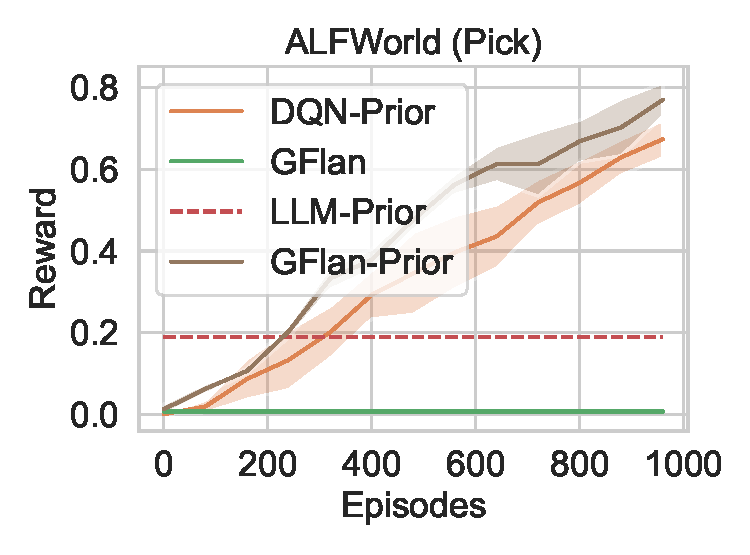
\includegraphics[width=0.30 \linewidth]{fig/train_curve_alf_pick_ab_new.pdf}
    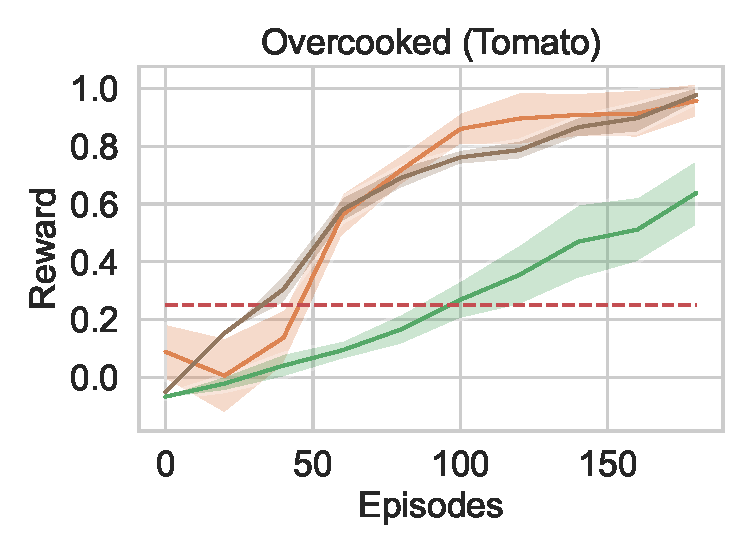
\includegraphics[width=0.30 \linewidth]{fig/train_curve_overcooked_ab_new.pdf}
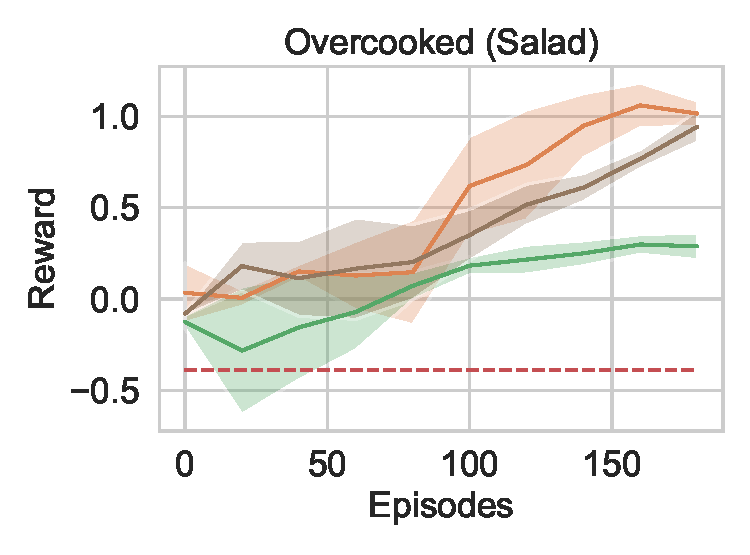
\includegraphics[width=0.30 \linewidth]{fig/train_curve_overcooked_lettuce_ab_new.pdf}
     }
     \subfigure[$k$ for GFlan-Prior]
      {    \label{gflank} 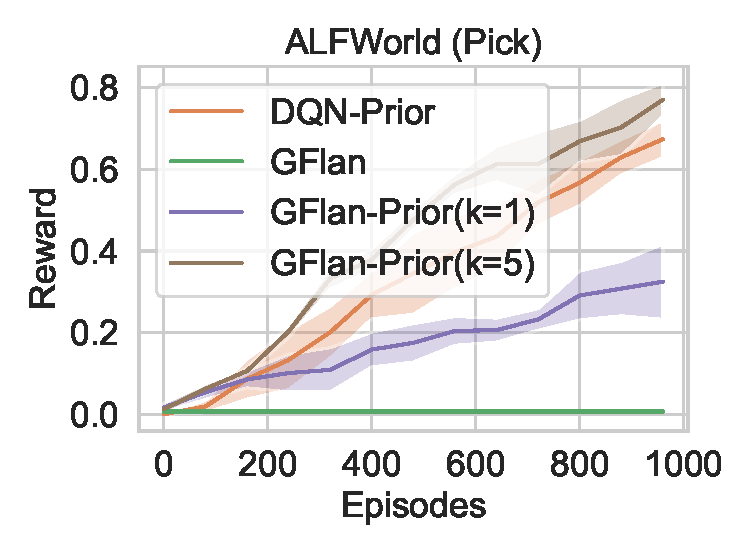
\includegraphics[width=0.30 \linewidth]{fig/train_curve_alf_pick_ab_newk.pdf}
     }
    \subfigure[$\alpha$ for GFlan-Prior]
      {    \label{gflanalpha} 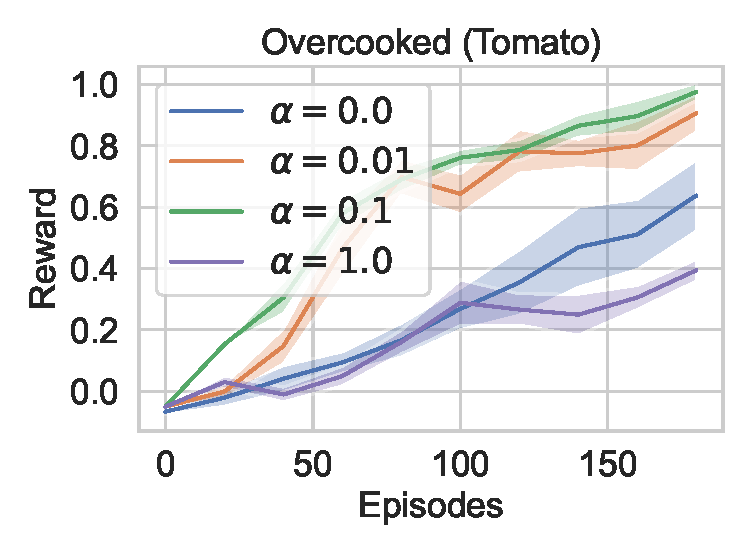
\includegraphics[width=0.30 \linewidth]{fig/train_curve_overcooked_ab_alpha_new.pdf}
     }
    \subfigure[$\alpha$ of DQN-Prior]{
\label{dqnalpha}  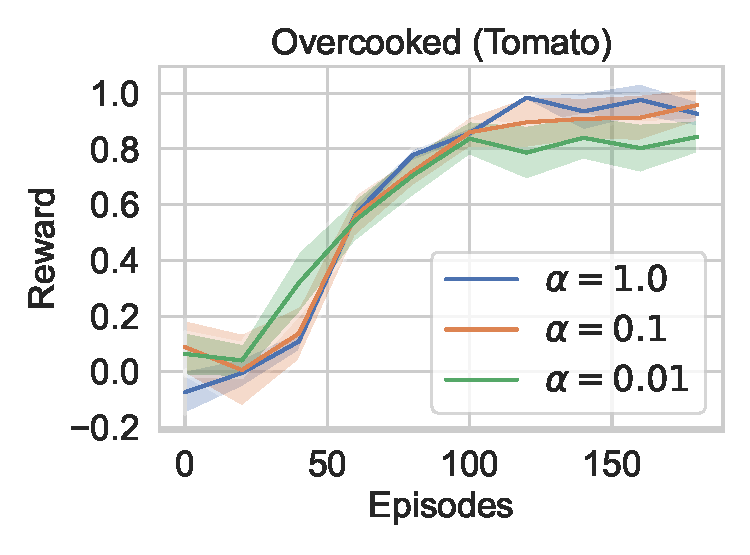
\includegraphics[width=0.30 \linewidth]{fig/train_curve_overcooked_alpha_value.pdf}		
    }
    \caption{(a) Comparison of policy-based RL algorithms, we plot DQN-Prior and LLM-Prior for reference. (b) The ablation study on the number of LLM action proposals $k$ used to approximate the KL divergence. (c) The ablation of the KL coefficient of GFlan-Prior. (d) The ablation of the softmax temperature over Q values of the DQN-Prior }%} 

\end{figure*}

\subsubsection{Incorporating LLM Priors into Policy-Based RL} The \fig \ref{fig:policy_base}, \ref{gflank}, \ref{gflanalpha} show the results of policy-based RL algorithms. As shown in Figure \ref{fig:policy_base}, GFlan-Prior significantly outperforms GFlan and achieves performance comparable to DQN-Prior. Unlike GFlan, GFlan-Prior leverages the prior knowledge embedded in LLMs by aligning with the LLM prior distribution through the incorporation of a KL constraint, as shown in Equation \ref{ppo}. In our main results, we sample $k=5$ action proposals from the LLM prior to approximate the KL divergence. An ablation study on $k$ can be found in Figure \ref{gflank} and Figure \ref{fig:policy_base_k} in the Appendix. Similar to the results in Table \ref{tab:generalize}, with $k=5$, we are more likely to sample the optimal action than with $k=1$, thereby better supervising the learning of the action policy. 
  
The ablation study on the coefficient of the KL divergence is shown in Figure \ref{gflanalpha}. A large $\alpha$ will cause the learned policy $\pi$ to closely follow the LLM prior proposals, while a small $\alpha$ encourages exploration. In DQN-Prior, the hyperparameter $\alpha$ regulates exploration by acting as the temperature in the softmax over Q, generating a Boltzmann distribution based on Q, as investigated in Figure \ref{dqnalpha}. GFlan-Prior appears to be more sensitive to the hyperparameter on controlling exploration than DQN-Prior.  
\section{Related Work}\label{Sec:RelatedWork}
% This work investigates combine Bayesian inference and LLMs for solving decision-making tasks. In this section, we introduce the probabilistic inference methods used in RL and the LLMs agent for decision making.
This study explores the fusion of Bayesian inference and LLMs for decision-making tasks. Herein, %\st{we present the probabilistic inference methods employed in RL and the LLM-based agent for decision-making tasks.} 
{we present related works on LLM-Agent for decision-making tasks and how previous research pursues this combination.} 

% \yan{(also, since our focus is from a RL side, I think the related work can go like this: 
% \begin{enumerate}
%     \item LLM + Probabilistic RL (most relevant)
%     \item resemblance to value-based inference
%     \item LLM-Agent (from a LLM side)
% \end{enumerate}
% }

%\paragraph{LLM Agent for Decision Making} There are several studies that investigate the leverage the LLMs to tackle decision-making (DM) tasks. These previous studies are roughly divided into three classes: prompt engineering-based, search based and fine-tuning-based LLM agents. Firstly, the prompt engineering-based methods, such as the Proagent \citep{zhang2023proagent}, Voyager \citep{wang2023voyager} and generative agents \citep{park2023generative}, directly use human deliberately design prompt to harness LLMs for complex interactive tasks, while the retrieval \citep{wang2023voyager,park2023generative} or rule-based controller \citep{zhang2023proagent} are used for complete decision-making tasks well.  Secondly, the search-based agent utilise the planning algorithm to find an optimal reasoning path for completing a long-term DM tasks. For instance, the Tree of Thought (ToT) \citep{yao2023tree} uses BFS/DFS algorithm to search the accurate decision sequence based on LLM assessment, and RAP \citep{hao2023reasoning} using the MCTS method to guide the reasoning generation process. ICPI \citepp{brooks2024large} use LLMs to serve as the world model and the rollout policy by in context learning, and rollout to estimate Q-value and then select the best action. 
% Although LLMs are able to generate human-understandable solutions for decision-making tasks, however, a careful grounding function is still required to align the output of LLMs with the action space.
% In order to achieve this purpose, LLMs %demonstrating strong in-context learning \citepp{min2022rethinking,rubin2021learning} ability 
% are 
%GFlan\citepp{carta2023grounding} ground the LLMs on solving a textual interactive task named BabyAI-Text, where the LLM Flan-T5 \citepp{rae2021scaling} is treated as the action policy and is fine-tuned via PPO \citepp{schulman2017proximal}. %, i.e., a  extension of BabyAI platform \citepp{chevalier2018babyai}. %which can be converted into textual RL settings via the extended BabyAI platform \citepp{chevalier2018babyai}, 
 {
\paragraph{LLM-driven Agent} The idea of LLM-as-Agent has gone viral since the release of powerful large language models. Among all the works, some apply direct prompt engineering techniques using human-designed prompt and retrieval to harness LLMs for complex interactive tasks, such as ProAgent by \citep{zhang2023proagent}, Voyager by \citep{wang2023voyager} and generative agent by \citep{park2023generative}. Many researchers have also tried searching-based methods. \citep{yao2023tree} propose Tree-of-Thought (TOT) using BFS/DFS algorithm to search accurate decision sequences. \citep{hao2023reasoning} suggests using Monte-Carlo Tree Search to perform a more comprehensive search. These methods often fall into the framework of Proposer-Verifier \citep{snell2024scaling} where the language proposes a number of possible sequences and the verifier picks desirable candidates. There are also a few works that relate LLM to conventional reinforcement learning settings and investigate how the superiority in language space helps RL agents' capability in decision-making. For instance, \citep{brooks2024large} uses LLM as a world model and performs policy iteration by in-context learning. GFlan proposed by \citep{carta2023grounding} uses a learnable LLM as a probability likelihood estimator for all possible actions and incorporates it into actor-critic learning frameworks where a value function generates assessment and fine-tuning the LLM correspondingly. \citep{yan2023ask} also resort to an actor-critic learning paradigm but instead of fine-tuning the language model, they train a simple classifier that selects valuable outputs from a fixed language model (e.g. GPT3.5). \citep{zhang2024can} use LLM as a behavior regularize and add it to the value estimate. \citep{wen2024entropy} leverages entropy-regularized reinforcement learning to train LLM agents for verbal sequential decision-making tasks. Our work also falls into the category of LLM-driven RL agent. However, different from others, we see a large language model as an excellent action proposer and perform Q-learning directly on the reformed action sequence space, thereby achieving better learning efficiency with minimum modification. 







}

% {
% \paragraph{Value-based Inference of LLM} Not limited to the pre-training phase, it has been recently investigated how scaling law applies at inference time for LLM. This is often referred to as searching over an enormously large output space with guidance from value estimation. For example, the naive case is beam search (citation) which selects the top K possible sequence based on cumulative probabilities as opposed to greedy search. The value estimate here is the likelihood of the sentence as predicted by the language model. \citep{wang2022self} propose CoT-SC, which searches over reasoning paths and selects the most frequent answer. Tree-of-Thought (ToT, \citep{yao2023tree}) adopts depth/breadth-first search. \citep{hao2023reasoning} introduce Reasoning-via-Planning (RAP) which uses Monte-Carlo Tree Search and value estimate from prompting LLM. TS-LLM designed by \citep{feng2023alphazero} guides MCTS with a learned value function conditioned on state and a learned Outcome-supervised Reward Model (ORM). \citep{li2024q} proposes Q-probing to adapt a pre-trained language model to also maximize a tasks-specific reward function in code generation tasks. Furthermore, recent works investigate Process-supervised Reward Model (PRM, \citep{lightman2023let}) and apply it in LLM inference, \citep{mcaleese2024llm} searches over a step-wise critic model in code reviewing tasks. \citep{wang2024math} learn a PRM in math reasoning and use it for LLM fine-tuning. \citep{snell2024scaling} provides a detailed benchmark of different inference methods. \citep{zhang2024generative} represents the score as the probability of a single text token (e.g. 'Yes' or 'No') under the context and the prompt. Even though our proposed method can be seen as an example of value-based inference, we focus on a different perspective where we investigate how LLM helps conventional value-based reinforcement learning algorithms in complex environments. More discussion can be found in Section \ref{sec: method}.

% }


{
\paragraph{LLM in Bayesian Sense}
The probabilistic nature of transformer-based language models makes them well-suited for a Bayesian inference framework. As highlighted by \citep{korbak2022rl}, the Bayesian approach offers a unified perspective on both modeling and inference. In in-context learning (ICL), some researchers argue for the Bayesian properties of ICL (\citep{jiang2023latent, wang2024large, ye2024pre}). Extending beyond ICL, \citep{yang2021fudge} trains a classifier to approximate the likelihood function, framing conditional text generation as a Bayesian inference problem, with the LLM serving as the prior. \citep{hu2023amortizing} interprets Chain-of-Thought (CoT) reasoning in natural language processing (NLP) tasks, such as text infilling and sequence continuation, as probabilistic inference problems, using GFlowNet to fine-tune the model. In this context, the language model functions as a unified probabilistic generative process, capable of representing both prior and likelihood distributions. Similarly, \citep{zhao2024probabilistic} adopts a Bayesian perspective, utilizing Sequential Monte Carlo (SMC) methods to generate undesired outcomes. \citep{gallego2024distilled} frames LLM inference as sampling from a posterior distribution focused on high-reward regions, applying this approach to self-improvement tasks. Inspired by these works, we also formulate our agent framework within a Bayesian setting, exploring the use of LLMs as priors.

% A transformer-based language model's probabilistic nature makes it easily applicable to a Bayesian inference framework. As noted by \citep{korbak2022rl}, the Bayesian view can 
% potentially provide a unified perspective on modeling and inference problems. The discussion of LLM in the Bayesian sense has started within the topics of in-context learning (ICL), where a few researchers argue on the Bayesian property of ICL (\citep{jiang2023latent, wang2024large, ye2024pre}). Beyond ICL, \citep{yang2021fudge} learns a classifier to mimic the likelihood function and formulate conditional text generation problems as Bayesian inference with LLM as a priori. \citep{hu2023amortizing} interpret CoT reasoning in NLP context such as text infilling and sequence continuation, as probabilistic inference problems and use GFlowNet to fine-tune the language model. In this case, a language model acts as a unified probabilistic generative process that is capable of describing both prior and likelihood distribution. \citep{zhao2024probabilistic} also holds a Bayesian view and leverages Sequential Monte Carlo (SMC) for generating undesired outcomes. \citep{gallego2024distilled} similarly frames LLM inference as sampling from a posterior distribution centered around high-reward regions, applying this approach to self-improvement tasks. Inspired by these efforts, we also formulate our agent framework within a Bayesian setting, exploring the potential of LLM as a priori.




% Probabilistic reinforcement learning (PRL) has a fairly large scope, and a transformer-based language model's probabilistic nature makes it easily applicable in the PRL context. 


% \paragraph{LLM as a probabilistic prior} From a probabilistic perspective, a large language model can be seen as a probabilistic generative process that outputs tokens autoregressive. This also

% }
}










\section{Conclusion}
%In this work, we are inspried by the remarkable suceess of LLMs on various domain attribute to their contained rich prior knowledge and powerful reasoning ability. 
In this work, we aim to leverage the rich domain knowledge and strong reasoning abilities of LLMs to solve complex decision-making tasks while avoiding the costly prompt design and fine-tuning of large language models. Given their rich prior knowledge but lack of task-specific experience, we do not rely on LLMs to directly output optimal plans. Instead, we focus on simplifying their role to generate reliable action proposals. Thus, we treat the powerful LLM as an action prior distribution and, from a Bayesian inference perspective, analyze how to incorporate LLM priors into solving MDPs. We utilize variational inference and posterior sampling to achieve this, ultimately proposing both policy-based and value-based frameworks with LLM priors. LLM priors improve traditional RL frameworks by reducing the exploration space or regulating the behavior of the action policy according to suboptimal LLM action proposals. Experimental results demonstrate a significant improvement in sample efficiency by incorporating fixed LLM priors into RL frameworks in both online and offline settings. This work focuses solely on text-based games with finite action spaces. In future work, we will explore scenarios with free-form and infinite action spaces, and try to incorporate prompt-based approaches to further enhance the quality of LLM prior action proposals.




\balance
\bibliography{ref}
\bibliographystyle{iclr2025_conference}
\section{Description of Classic Q-learning Algorithm}
We introduce the classic Q-learning algorithm in both offline and online settings.
\paragraph{Q-learning}
Q-learning is a classic value-based RL algorithm, which iteratively applies the Bellman optimal operator to train the Q-function, formally written as $\mathcal{B}^*Q(s,a)=r(s,a)+\gamma \mathbb{E}_{s^\prime\sim P(\cdot|s,a)}\left[\max_a^\prime Q(s^\prime,a^\prime)\right]$. After the optimal Q-function $Q^*$ learned, then the optimal action policy respect to the $Q^*$ is given as: $\pi^*(\cdot|s)=\arg\max_a Q^*(s,a)$. DQN \citep{mnih2013playing} is a well-known Q-learning algorithm, which can process various classes of the state information such as image and language, which learns a deep neural network $Q^\theta(s,a)\approx Q^*(s,a)$ to approximate $Q^*(s,a)$ and uses TD-learning to iteratively update the Q network, the loss function for the $i$-the iteration is given as: 
\begin{equation}
\mathcal{L}_i(\theta)=\mathbb{E}_{(s,a,s^\prime)\sim \mathcal{D}}\left[(Q^{\theta_i}(s,a)-y_i)^2\right],
\end{equation}
where $\mathcal{D}$ is the reply buffer, $y_i=\mathcal{B}^*Q^{\theta_{i-1}}(s,a)=r(s,a)+\gamma \max_{a^\prime\in \mathcal{A}} Q^{\theta_{i-1}}(s^\prime,a^\prime)$. $\theta_{i-1}$ is the learned parameters of the last iteration and is frozen during the gradient descent for optimizing the loss function $\mathcal{L}_i$.
\paragraph{Conservative Q-learning}
CQL \citep{kumar2020conservative} framework is designed for offline reinforcement learning, where only offline data is available, but no further online exploration is accessible. Different from traditional Q-learning, CQL introduces an additional regularization term on top of the standard DQN framework or actor-critic framework(such as SAC \citep{haarnoja2018soft}), ensuring that the learned Q-function lower-bounds the actual value. The lower-bounded Q-values help mitigate the overestimation problem commonly encountered with out-of-distribution (OOD) state-action pairs. The CQL loss on the top of value-based DQN is given as:
\begin{equation}
\mathcal{L}_i(\theta)=\beta\mathbb{E}_{(s,a)\sim \mathcal{D}}\left[\log \sum_{a^\prime\in \mathcal{A}} \exp(Q^{\theta_i}(s,a^\prime))-Q^{\theta_i}(s,a)\right]+\frac{1}{2}\mathbb{E}_{(s,a,s^\prime)\sim \mathcal{D}} \left[(Q^{\theta_i}(s,a)-y_i)^2\right],
\end{equation}
where $y_i=r(s,a)+\gamma \max_{a^\prime} Q^{\theta_{i-1}}(s^\prime,a^\prime)$ and $\beta$ is a hyper-parameter.


\section{Proofs}

\subsection{Probabilistic Inference Derivation}\label{appendix: probabilistic}
In this section, we derive the detailed formulation for probabilistic inference for using LLM as a prior. This includes the policy-based method where we learn a parametrized policy function and the value-based method where we directly perform posterior inference.

\paragraph{Variational Inference}
 Assume that we have the optimality variable $\mathcal{O}$ indicating the quality of a trajectory $\tau = \{s_0, a_0, r_0, s_{1}, ..., s_n \}, p(\tau) = p(s_0)\prod_t p(a_t|s_t)p(s_{t+1}|s_t, a_t)$. The likelihood function with temperature parameter $\alpha$ can be written as:
\begin{equation}
    p(\mathcal{O}=1|\tau) = \exp \left(\sum_t \gamma^tr_t/\alpha \right)
\end{equation}
Our goal is to maximize the optimal marginal distribution formulated as follows:
\begin{equation}
\begin{aligned}
    p(\mathcal{O}=1) & =  \int p(\mathcal{O}=1, \tau) d\tau \\
    & = \int q(\tau) \frac{p(\mathcal{O}=1|\tau)p(\tau)}{q(\tau)} d\tau 
\end{aligned}
\end{equation}
where $q(\tau)$ is a parametrized variational distribution. Then, our variational inference objective can be written as:
\begin{equation}
\begin{aligned}
\log p(\mathcal{O}=1) & \geq \int q(\tau) \log \left[p(\mathcal{O}=1|\tau) \frac{p(\tau)}{q(\tau)} \right] d\tau \\
& = \mathbb{E}_{q(\tau)}\left[\log p(\mathcal{O}=1|\tau) \right] - \textbf{KL}\left[q(\tau) | p(\tau)\right] \\
& = \textbf{ELBO}
\end{aligned}
\end{equation}
In the context of language models, we define prior $p(\tau)$ as trajectory distribution generated through a fixed LLM denoted as:
\begin{equation}\label{eq: llm prior}
    p_{LLM}(\tau) = p(s_0)\prod_t p_{LLM}(a_t|s_t)p(s_{t+1}|s_t, a_t)
\end{equation}
where $p_{LLM}(a_t|s_t)$ is the probability likelihood of the generated output $a_t$ given input text $s_t$. The variational distribution $q(\tau)$ can also be decomposed in the same way as:
\begin{equation}
    q(\tau) = p(s_0)\prod_t \pi_{\theta}(a_t|s_t)p(s_{t+1}|s_t, a_t)
\end{equation}
where the parametrized policy function $\pi_{\theta}$ can be a learnable language model with parameter $\theta$. Substituting these factorizations back to ELBO we have the step-wise objective function written as:
\begin{equation}
    -\mathcal{L} = \sum_{t} \mathbb{E}_{\pi_{\theta}}\left[\gamma^t r_t \right] - \alpha \textbf{KL}\left[ \pi_{\theta}(a_t|s_t) \| p_{LLM}(a_t|s_t) \right]
\end{equation}
\begin{equation}
    \pi^{*} = \argmin_{\theta} \mathcal{L}
\end{equation}



\paragraph{Direct Posterior Inference} Instead of learning a parametrized policy which might involve fine-tuning a language model, we can also try directly sampling from the posterior distribution formulated as:
\begin{equation}
\begin{aligned}
     p(\tau|\mathcal{O}=1) & = \frac{p(\mathcal{O}=1|\tau)p(\tau)}{p(\mathcal{O}=1)}\\
     & \propto p(\mathcal{O}=1|\tau)p(\tau) \\
     & = \prod_{t}p(\mathcal{O}_t=1|s_t, a_t)p_{LLM}(a_t|s_t)p(s_{t+1}|s_{t}, a_t)
\end{aligned}
\end{equation}
in which we define $p(\tau)$ as in Equation \ref{eq: llm prior}. According to Control-as-Inference framework proposed by \cite{levine2018reinforcement}, we can formulate posterior inference as Soft Q-Learning where Q-values are updated using a modified soft Bellman equation:
\begin{equation}
\begin{aligned}
    Q^{\pi}(s_t, a_t) = r(s_t, a_t) + \gamma \mathbb{E}_{s_{t+1}\sim p(\cdot|s_t, a_t)}\left[V(s_{t+1}) \right] \\
    V(s_t) = \log\int \exp (Q(s_t, a_t)/\alpha) da_t
\end{aligned}
\end{equation}
and the policy can be defined as a softmax function over the Q-values: $\pi(a|s) = \exp(Q^{\pi}(s,a)/\alpha) / \int_{a^{'}} \exp(Q^{\pi}(s,a^{'})/\alpha) da^{'}$, ensuring that actions with higher Q-values are more likely to be chosen. In our paper, however, due to the enormously large space of (textual) state-action pair, we also apply sampling approximation methods. Specifically, we leverage similar ideas from \cite{fourati2024stochastic} which sample a random subset of actions from the complete action space and seek the optimal within this subset. In our case, we rely on a fixed LLM to provide such action subspace and can further narrow down the space through repeated sampling (\cite{brown2024large}):
% through repeated sampling (\cite{brown2024large}):
\begin{equation}
\begin{aligned}
    \pi(a|s) & = \frac{\mathbf{1}_{a \in p_{LLM}(\cdot|s) } \cdot \exp\left(Q^{\pi}(s, a)/\alpha\right)}{
    \int_{a^{'}} \mathbf{1}_{a \in p_{LLM}(\cdot|s) } \cdot \exp\left(Q^{\pi}(s, a^{'})/\alpha\right) da^{'}
    } \\
    & \approx \mathbf{1}_{a\in\{a^i\}} \cdot \frac{1}{N} \frac{\exp(Q^{\pi}(s, a^{i})/\alpha)}{\sum_{i}\exp(Q^{\pi}(s, a^{i})/\alpha)}, a^i \sim p_{LLM}(a|s)
\end{aligned}
\end{equation}
This means we restrict the Bellman backup to a specific action subspace that can potentially provide a refined set of actions based on context, largely reducing computational complexity and focusing on more relevant actions.





% and aim to learn a step-wise scoring function $f(s,a)$ taking state-action pair in textual MDP and approximating the likelihood distribution $p(\mathcal{O}=1|\tau)$.



\subsection{Proof of Proposition \ref{proposition}}
\propsa*
\begin{proof}
The proof mainly follows the \citep{li2024q}. Denote the above sampling strategy indeed follows a distribution $q$, and for each action $a$, the probability of $a$ is sampled from the distribution $q$ is given by:
\begin{equation}
    %\lim_{k\rightarrow\infty} ()
    \begin{aligned}
            q(a|s_t)&=\mathbb{E}_{\{a_1,\cdots,a_k\}\sim p_\text{LLM}(\cdot|s)}\left[\sum_{i=1}^k \mathbb{I}(a_i=a) \frac{\exp( Q^\theta(s_t,a_i)/\alpha)}{\sum_{j=1}^k \exp( Q^\theta(s_t,a_j)/\alpha)}\right]\\
            &=\mathbb{E}_{\{a_1,\cdots,a_k\}\sim p_\text{LLM}(\cdot|s)}\left[ \frac{\sum_{i=1}^k \mathbb{I}(a_i=a)}{\sum_{j=1}^k \exp( Q^\theta(s_t,a_j)/\alpha)}\right]\exp( Q^\theta(s_t,a)/\alpha)\\
            &=\mathbb{E}_{\{a_1,\cdots,a_k\}\sim p_\text{LLM}(\cdot|s_t)}\left[ \frac{\frac{1}{k}\sum_{i=1}^k \mathbb{I}(a_i=a)}{\frac{1}{k}\sum_{j=1}^k \exp( Q^\theta(s_t,a_j)/\alpha)}\right]\exp( Q^\theta(s_t,a)/\alpha)\\
    \end{aligned}
\end{equation}
According to the Law of Large Numbers, when $k\rightarrow \infty$, we have:
\begin{equation}
\begin{aligned}
        \lim_{k\rightarrow\infty} q(a|s_t)&= \lim_{k\rightarrow\infty} \mathbb{E}_{\{a_1,\cdots,a_k\}\sim p_\text{LLM}(\cdot|s_t)}\left[ \frac{\frac{1}{k}\sum_{i=1}^k \mathbb{I}(a_i=a)}{\frac{1}{k}\sum_{j=1}^k \exp( Q^\theta(s_t,a_j)/\alpha)}\right]\exp( Q^\theta(s_t,a)/\alpha)\\
        &= \lim_{k\rightarrow\infty} \mathbb{E}_{\{a_1,\cdots,a_k\}\sim p_\text{LLM}(\cdot|s_t)}\left[ \frac{p_\text{LLM}(a|s_t)}{\mathbb{E}_{a_j \sim p_\text{LLM}(\cdot|s_t)} \exp( Q^\theta(s_t,a_j)/\alpha)}\right]\exp( Q^\theta(s_t,a)/\alpha)\\
        &= p_\text{LLM}(a|s_t)\frac{\exp( Q^\theta(s,a)/\alpha)}{\mathbb{E}_{a_j \sim p_\text{LLM}(\cdot|s)} \exp( Q^\theta(s,a_j)/\alpha)}
\end{aligned}
\end{equation}
Following the proof process from the Appendix A.1. in \cite{rafailov2023direct}, we have:
\begin{equation}
\label{dpo}
    \arg\max _\pi \mathbb{E}_{\pi(a|s_t)} [Q^\theta(s_t,a)]-\alpha \text{KL}\left(\pi(\cdot|s_t)\|p_\text{LLM}(\cdot|s_t)\right)=p_\text{LLM}(a|s_t)\frac{\exp( Q^\theta(s,a)/\alpha)}{\mathbb{E}_{a_j \sim p_\text{LLM}(\cdot|s)} \exp( Q^\theta(s,a_j)/\alpha)}
\end{equation}
\end{proof}

Additionally, as shown in Sec. \ref{sec: method}, the variational inference approach learns the optimal policy $\pi$ by maximising:
\begin{equation}
\label{variation_appen}
%\arg\max_\pi \mathcal{J}(\pi) = 
\arg\max_\pi \sum_t  \mathbb{E}_\pi\left[\gamma^t r_t\right] - \alpha \, \text{KL}(\pi(a|s_t) \| p_{\text{LLM}}(a|s_t)).
\end{equation}
Introducing the occupancy measure $\rho$, $\rho(s)=\frac{1}{1-\gamma}\sum_{t=0}^\infty [\gamma^t \mathbb{P}(s_t=s|a\sim \pi)]$, we have the following form objective respected to the Q-function
\begin{equation}
\label{optq}
\arg\max_\pi \mathbb{E}_{\rho(s)}[\mathbb{E}_{a\sim\pi}[Q^\pi(s,a)]-\alpha \text{KL}(\pi(a|s_t) \| p_{\text{LLM}}(a|s_t))]
\end{equation}
Combining Equations \ref{dpo} and \ref{optq}, we find that the variational inference approach and the direct posterior sampling yield similar solutions.
\section{Additional Experiment Details}
\subsection{Environments}

We consider three environments:
\newline\textbf{ALFWorld} %This game connects the text-based world of TextWorld with the parallel embodied worlds in the ALFRED dataset. 
 We consider two classes of ALFWorld tasks: ALFWorld(pick) and ALFWorld(examine). For ALFWorld (Pick), we evaluate the online training baselines on 28 tasks, such as "put the cellphone on the armchair," and test the generalization ability on 26 unseen tasks. For ALFWorld (Examine), we use 11 tasks, such as "examine the laptop with the desk lamp." There are no auxiliary rewards, except for a reward of $1.0$ for reaching the final goal. 
\newline\textbf{Overcooked} We use the partially observed text overcooked game; the observation describes the position of visible items, and the agent should take a sequence of actions to deliver a dish. We consider two overcooked tasks: Overcooked(Tomato), deliver a dish of chopped tomato; Overcooked(Salad), deliver a salad containing chopped tomato and lettuce. The maximum possible action space is $8$. Besides the reward of $1$ for successfully delivering a dish, the textual Overcooked environment from \cite{tantrue} also provides dense reward signals. The reward shaping is as follows: 0.2 for correctly chopping an ingredient, 1 terminal reward for successfully delivering the correct dish, $-0.1$ for delivering any incorrect item, and $-0.001$ for each time step.
\newline\textbf{Frozen Lake} is a grid world game; the agent should move to the goal position while avoiding full into holes. There are four admissible actions: up, down, right, and left. The agent will receive a reward of $1$ for reaching the final goal and a penalty of $-1$ for falling into holes. The maximum steps for these three tasks are shown in Table \ref{tab:horizon}.
\begin{table}[]
    \centering
    \begin{tabular}{c|ccccc}
    \hline
         & ALFWorld(Pick) &ALFWolrd(Examine) &Cook(Tomato)&Cook(Salad) &Frozen Lake  \\
         \hline
         Horizon& 60&60&30&50&20 \\
         \hline
    \end{tabular}
    \caption{Maximize horizon of environments. }
    \label{tab:horizon}
\end{table}

\subsection{LLM prior implementation}
There are two ways to sample an action $a$ from the LLM prior $p_{\text{LLM}}(\cdot | s_t)$. First, since the state and action can be described as text, and assuming the action $a$ consists of $k$ tokens, the probability of the LLM generating action $a$ is given by $p(a | s_t) = \prod_{i=1}^k p_{\text{LLM}}(a_i | s_t, a_{<i})$. Based on this probability, the first type of LLM prior computes a distribution over actions, denoted as $p_{\text{LLM}}^{\text{dist}}(a | s_t) = \frac{\exp p(a | s_t)}{\sum_{a^\prime} \exp p(a^\prime | s_t)}$. In contrast, the second approach involves sampling a free-form output from the LLM, which is then mapped to an executable action via a simple rule-based projection $\mathcal{P}$. We denote this LLM prior, which relies on mapping the LLM's output, as $p_{\text{LLM}}^{\text{map}}$, where $a \sim p_{\text{LLM}}^{\text{map}}(\cdot | s_t) \leftrightarrow o \sim \text{LLM}(\cdot | s_t), a = \mathcal{P}(o)$.


%The KL-divergence encourages the learned policy \(\pi\) to stay close to the powerful LLM prior, which is often powerful. In practice, the cumulative reward is straightforward to compute by rolling out an entire trajectory. For computing the KL-divergence, LLM-based RL approaches \cite{carta2023grounding, wen2024entropy} can either: 1) directly compute the distribution over action in the form of $p_{\text{LLM}}^{\text{dist}}$, or 2) simplify the KL computation by focusing solely on a sample from \(p^\text{map}_{\text{LLM}}(a|s_t)\), where actions generated with high probability by the LLM prior are more likely to be selected \cite{zhang2024can}.


We observed a performance gap between these two types of LLM action priors. For instance, in the ALFWorld pick \& place task, $p_{\text{LLM}}^{\text{map}}$ achieved a winning rate of $19\%$, while $p_{\text{LLM}}^{\text{dist}}$ failed, with a winning rate of $0\%$, both using the LLM Qwen1.5-7B. Therefore, in this work, we implement $p_{\text{LLM}}^{\text{map}}$ as the LLM prior for thoughtfully exploiting the power of the LLM in SDM tasks, which we denote as $p_{\text{LLM}}$ for simplicity.
Examples of LLM's output is given as:
\begin{tcolorbox}[title={For ALFWorld(Pick) from Qwen-1.5 7B}]
    
\textbf{Input:}
Current observation:You are in the middle of a room. Looking quickly around you, you see a armchair 1, a bed 1, a diningtable 1, a drawer 2, a drawer 1, a garbagecan 1, a sidetable 2, and a sidetable 1.

Your task is to: put some cellphone on armchair.. You are allowed to take the following actions: go to armchair 1, go to bed 1, go to diningtable 1, go to drawer 1, go to drawer 2, go to garbagecan 1, go to sidetable 1, go to sidetable 2, inventory, look.
Please select an action from the admissible actions. 

\textbf{Output:} 
1: take cd 2 from sidetable 2 , 

2: Open drawer 2 Result: You open door, 

3: look Description: You look around the room., 

4: look > Current observation:You arrive at loc, 

5: open drawer 2 Loc 8: You

\end{tcolorbox}
\subsection{Hyper-parameters}
Our algorithms are trained on one machine with $2$ 40G A100. based on Pytorch-GPU 2.1 and cuda12.4. Table \ref{tab:tomato},\ref{tab:salad},\ref{tab:lake},\ref{tab:pick},\ref{tab:exam} reports the main hyper-parameters of our algorithms. For all CQL-based algorithms, we set the hyperparameter $\beta$ for regulating the Q-values, as shown in \eq \ref{cql_loss}, as $5.0$.
\paragraph{Offline Datasets}
The composition of offline datasets is shown in Table \ref{tab:offline_data}, which reports the number of $(s,a,s^\prime)$ examples.

\begin{table}[]
    \caption{The hyperparameters on ALFWorld(Pick)}
    \centering
    \begin{tabular}{cccccccc}
    \hline
    Baselines & Learning Rate & Epochs & Batch Size & Update Frequency& LLM &$\alpha$\\
    \hline
        DQN-Prior & 5e-4& 4&128&5&/ &0.01  \\
        CQL-Prior & 5e-4& 4&128&5  &/ &0.01 \\
        GFlan-Prior  & 1e-4& 16&64&16&Flan-T5 Small&0.01  \\
    \hline
        \end{tabular}
    \label{tab:paralake}
\end{table}
\begin{table}[]
    \caption{The hyperparameters on ALFWorld(Examine)}
    \centering
    \begin{tabular}{cccccccc}
    \hline
    Baselines & Learning Rate & Epochs & Batch Size & Update Frequency& LLM &$\alpha$\\
    \hline
        DQN-Prior & 5e-4& 4&128&10&/ &0.01  \\
        CQL-Prior & 5e-4& 4&128&10  &/ &0.01 \\
        GFlan-Prior  & 1e-4& 16&64&16&Flan-T5 Small&0.01  \\
    \hline
        \end{tabular}
    \label{tab:paralake}
\end{table}
\begin{table}[]
    \caption{The hyperparameters on Overcooked(Tomato
    )}
    \centering
    \begin{tabular}{cccccccc}
    \hline
    Baselines & Learning Rate  & Batch Size & Update Frequency& LLM &$\alpha$\\
    \hline
        DQN-Prior & 5e-4&128&5&/ &0.1  \\
        CQL-Prior & 5e-4&128&5  &/ &0.1 \\
        GFlan-Prior  & 1e-4&64&16&Flan-T5 Small&0.1  \\
    \hline
        \end{tabular}
    \label{tab:tomato}
\end{table}
\begin{table}[]
    \caption{The hyperparameters on Overcooked(Salad)}
    \centering
    \begin{tabular}{cccccccc}
    \hline
    Baselines & Learning Rate  & Batch Size & Update Frequency& LLM &$\alpha$\\
    \hline
        DQN-Prior & 5e-4&128&5&/ &0.1  \\
        CQL-Prior & 5e-4&128&5  &/ &0.1 \\
        GFlan-Prior  & 1e-4&64&16&Flan-T5 Small&0.1  \\
    \hline
        \end{tabular}
    \label{tab:salad}
\end{table}
\begin{table}[]
    \caption{The hyperparameters on Frozen Lake}
    \centering
    \begin{tabular}{cccccccc}
    \hline
    Baselines & Learning Rate  & Batch Size & Update Frequency& LLM &$\alpha$\\
    \hline
        DQN-Prior & 5e-4& 128&5&/ &0.1  \\
        %CQL-Prior & 5e-4& 4&128&5  &/ &0.1 \\
        %GFlan-Prior  & 1e-4& 16&128&64&Flan-T5 Small&0.1  \\
    \hline
        \end{tabular}
    \label{tab:lake}
\end{table}
\begin{table}[]
    \caption{The hyperparameters on ALFWorld(Pick)}
    \centering
    \begin{tabular}{cccccccc}
    \hline
    Baselines & Learning Rate  & Batch Size & Update Frequency& LLM &$\alpha$\\
    \hline
        DQN-Prior & 5e-4&128&10&/ &0.01  \\
        CQL-Prior & 5e-4&128&10  &/ &0.01 \\
        GFlan-Prior  & 1e-4&64&16&Flan-T5 Small&0.01  \\
    \hline
        \end{tabular}
    \label{tab:pick}
\end{table}
\begin{table}[]
    \caption{The hyperparameters on ALFWorld(Examine)}
    \centering
    \begin{tabular}{cccccccc}
    \hline
    Baselines & Learning Rate  & Batch Size & Update Frequency& LLM &$\alpha$\\
    \hline
        DQN-Prior & 5e-4&128&10&/ &0.01  \\
        CQL-Prior & 5e-4&128&10  &/ &0.01 \\
        GFlan-Prior  & 1e-4&64&16&Flan-T5 Small&0.01  \\
    \hline
        \end{tabular}
    \label{tab:exam}
\end{table}
\begin{table}[]
    \centering
    \begin{tabular}{c|ccc}
    \hline
         Dataset & Total Examples & Good Examples & Bad Examples  \\
         \hline
         ALFWorld(Pick)&6572&6572&0 \\
         Salad(1000)&1186&574&612\\
         Salad(4000)&3892&2209&1683\\
         Salad(8000) &7571&4224&3347\\
         Salad(12000)&11939&4004&7935\\
           Salad(24000)&23869&7191&16678\\
\hline
    \end{tabular}
    \caption{The composition of the offline dataset}
    \label{tab:offline_data}
\end{table}
\subsection{Additional Results}
\begin{figure*}[t!]
%  \vspace{-0.5em}
	\centering
 % \includegraphics[width=1.0 \linewidth]{fig/legendablation.pdf}
	{
 
%
\includegraphics[width=0.35 \linewidth]{fig/legendbaselineprior_policy.pdf}
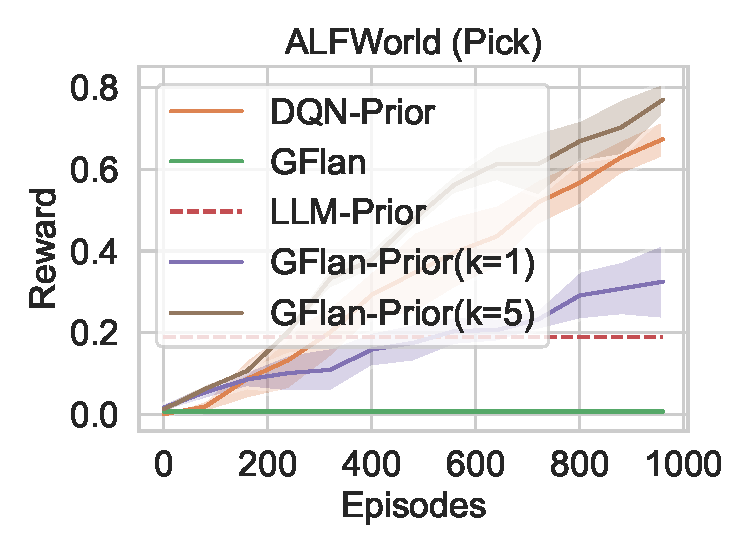
\includegraphics[width=0.28 \linewidth]{fig/train_curve_alf_pick_ab.pdf}
    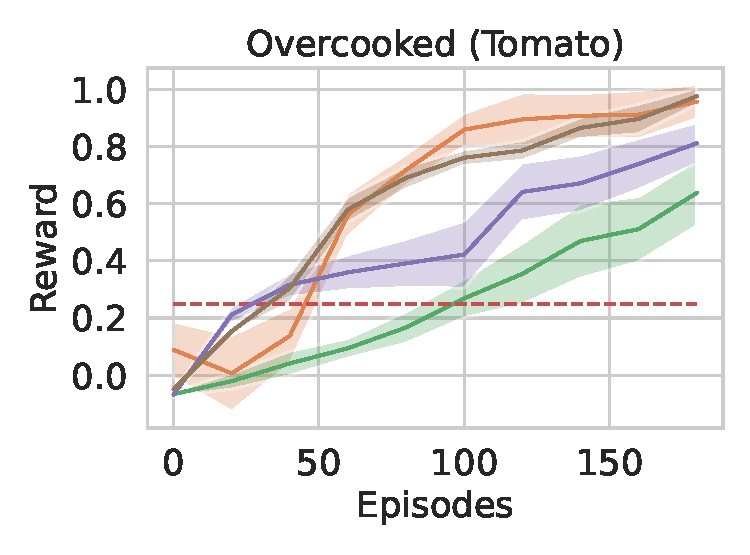
\includegraphics[width=0.28 \linewidth]{fig/train_curve_overcooked_ab.pdf}
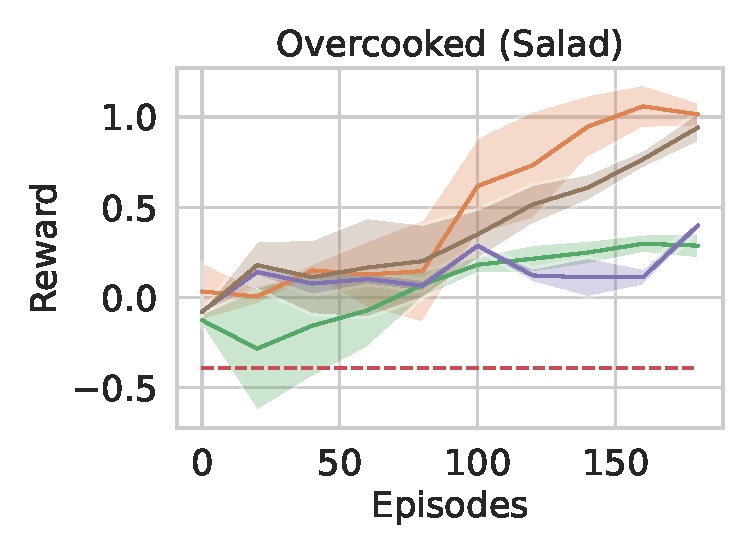
\includegraphics[width=0.28 \linewidth]{fig/train_curve_overcooked_lettuce_ab.pdf}
     }
    
    \caption{The ablation of the number of action proposals $k$ used for approximating KL divergence between the required action policy and the LLM prior action distribution.}%} 
\label{fig:policy_base_k}
\end{figure*}

\paragraph{Additional ablation on $k$ for GFlan-Prior} As shown in \fig \ref{fig:policy_base_k}, when we sample $k=5$ action proposals from the LLM to approximate the KL divergence, it performs better than when using $k=1$. This is because, with more proposals, the optimal action is more likely to be included in the subset, thus better guiding the action policy.

\section{Additional Related Works}\label{sec: extra related works}
\paragraph{Value-based Inference of LLM} Not limited to the pre-training phase, it has been recently investigated how scaling law applies at inference time for LLM. This is often referred to as searching over an enormously large output space with guidance from value estimation. For example, the naive case is beam search (citation) which selects the top K possible sequence based on cumulative probabilities as opposed to greedy search. The value estimate here is the likelihood of the sentence as predicted by the language model. \citep{wang2022self} propose CoT-SC, which searches over reasoning paths and selects the most frequent answer. Tree-of-Thought (ToT, \citep{yao2023tree}) adopts depth/breadth-first search. \citep{hao2023reasoning} introduce Reasoning-via-Planning (RAP) which uses Monte-Carlo Tree Search and value estimate from prompting LLM. TS-LLM designed by \citep{feng2023alphazero} guides MCTS with a learned value function conditioned on state and a learned Outcome-supervised Reward Model (ORM). \citep{li2024q} proposes Q-probing to adapt a pre-trained language model to also maximize a tasks-specific reward function in code generation tasks. Furthermore, recent works investigate Process-supervised Reward Model (PRM, \citep{lightman2023let}) and apply it in LLM inference, \citep{mcaleese2024llm} searches over a step-wise critic model in code reviewing tasks. \citep{wang2024math} learn a PRM in math reasoning and use it for LLM fine-tuning. \citep{snell2024scaling} provides a detailed benchmark of different inference methods. \citep{zhang2024generative} represents the score as the probability of a single text token (e.g. 'Yes' or 'No') under the context and the prompt. Even though our proposed method can be seen as an example of value-based inference, we focus on a different perspective where we investigate how LLM helps conventional value-based reinforcement learning algorithms in complex environments. More discussion can be found in Section \ref{sec: method}.

\iffalse
\section{Reproducibility Statement}
We have provided a detailed description of the algorithm and reported the key hyperparameters and LLM configurations. We are committed to making our code publicly available upon acceptance of the paper.
\fi

% \bibliographystyle{plain}
% \bibliography{ref}
\end{document}